%Preamble
\documentclass[11pt,oneside,letterpaper]{report}

%Page formatting package
\usepackage[top=1.0in, bottom=1in, left=1.5in, right=1in]{geometry}
\usepackage{setspace}
%Double spacing
\linespread{1.5}
%Graphics package
\usepackage{graphicx}
\DeclareGraphicsExtensions{.png,.jpg,.pdf}
%For multirow feature to draw tables
\usepackage{multirow}
%Middle allignment in tables.
\usepackage{array}
%For Mathematics
\usepackage{amsmath}
\numberwithin{equation}{section}
%Float package used to specify positioning
\usepackage{float}
%Depth of upto four in sections.
%\setcounter{secnumdepth}{3}

\usepackage{algorithmic}
\usepackage{algorithm}
\numberwithin{algorithm}{chapter}

%Reformat current date and time
\usepackage{datetime}

%For hyper referencing
\usepackage[pdfborder={text},colorlinks={true},linkcolor={black},citecolor={black},urlcolor={black}]{hyperref}
%In case you use the package hyperref to create a PDF, the links to tables or figures will point to the caption of the table or figure, which is always below the table or figure itself. Therefore the table or figure will not be visible, if it is above the pointer and one has to scroll up in order to see it. If you want the link point to the top of the image you can use the package hypcap with:
\usepackage[all]{hypcap}

\usepackage[acronym]{glossaries}
\makeglossaries
\newacronym{al}{AL}{Artificial Life}
\newacronym{ca}{CA}{Cellular Automata}
\newacronym{cas}{CAS}{Complex Adaptive System}
\newacronym{ea}{EA}{Evolutionary Algorithm}
\newacronym{ec}{EC}{Evolutionary Computation}
\newacronym{ep}{EP}{Evolutionary Programming}
\newacronym{es}{ES}{Evolutionary Strategies}
\newacronym{formal}{FormAL}{Formal Artificial Life}
\newacronym{ga}{GA}{Genetic Algorithm}
\newacronym{gp}{GP}{Genetic Programming}
\newacronym{rna}{RNA}{Ribonucleic Acid}

%Preamble ends document begins
\begin{document}

\begin{titlepage}
\begin{center}

\LARGE \textbf{Modeling the Evolution of Mimicry}\\[1.5cm]
\large \textbf{Mohiul Islam}\\[2.5cm]
\large A Thesis\\ in\\ The Department\\ of\\ Computer Science\\ and Software Engineering\\[2.5cm]
\large Presented in Partial Fulfillment of the Requirements\\ for the Degree of Master of Computer Science at\\ Concordia University\\ Montreal, Quebec, Canada\\[1.5cm]
\large \monthname \ \the \year \\[2cm]
\vfill
\large \copyright \ Mohiul Islam, \the \year
\end{center}
\end{titlepage}

%\newpage
\begin{titlepage}
\begin{center}
\Large \textbf{CONCORDIA UNIVERSITY}\\
\Large \textbf{School of Graduate Studies}\\[1cm]
\end{center}
This is to certify that the thesis prepared\\
\makebox[1.6in][l]{By:} Mohiul Islam\\
\makebox[1.6in][l]{Entitled:}  Modeling the Evolution of Mimicry\\
and submitted in partial fulfillment of the requirements for the degree of
\begin{center}
\small \textbf{Master of Computer Science}\\
\end{center}
complies with the regulations of the University and meets the accepted standards with respect to originality and quality.\\[0.4cm]
\begin{spacing}{1}
\noindent
Signed by the final examining committee:\\[0.8cm]
\makebox[5cm][l]{} \rule{7cm}{0.1mm} Chair\\ 
\makebox[5cm][l]{} Dr. E. J. Doedel\\[0.8cm]
\makebox[5cm][l]{} \rule{7cm}{0.1mm} Examiner\\ 
\makebox[5cm][l]{} Dr. T. Radhakrishnan\\[0.8cm]
\makebox[5cm][l]{} \rule{7cm}{0.1mm} Examiner\\ 
\makebox[5cm][l]{} Dr. N. Kharma\\[0.8cm]
\makebox[5cm][l]{} \rule{7cm}{0.1mm} Supervisor\\ 
\makebox[5cm][l]{} Dr. P. Grogono\\[0.8cm]
\makebox[5cm][l]{Approved by} \rule{10cm}{0.1mm}\\ 
\makebox[5cm][l]{} Chair of Department or Graduate Program Director\\[0.8cm]
\makebox[5cm][l]{} \rule{10cm}{0.1mm}\\ 
\makebox[5cm][l]{} Dr. Robin A. L. Drew, Dean \\
\makebox[5cm][l]{} Faculty of Engineering and Computer Science\\[0.8cm]
\makebox[5cm][l]{Date} \rule{7cm}{0.1mm}
\end{spacing}
\end{titlepage}
\pagenumbering{roman}

\newpage
\begin{center}

\Large \textbf{Abstract}\\[0.5cm]
\large \textbf{Modeling the Evolution of Mimicry}\\
\small \textbf{Mohiul Islam}\\

\end{center}

A novel agent based, artificial life model, for the evolution of mimicry is presented. This model is a predator-prey co-evolution scenario where pattern representation phenotype is simulated with Cellular Automata, while behaviors of pattern recognition is configured with Hopfield Network. A visual three dimensional toroidal cube is used to construct a universe in which agents have complete freedom of mobility, genetic representation of behavior and reproduction capability to evolve new behaviors in successive generations. These agents are classified into categories of predator and prey species. Genome of prey species control their mobility and palatability, while 2D Cellular Automata (CA) is used to represent a pattern, where the rule to generate the CA is also genetically represented. Through evolution, successive generations of prey species have new pattern to represent them both visually and to the predators. Predators are agents with the primary purpose of providing selection pressure for the evolution of mimicry. They are equipped with Hopfiled Network memory to recognize new CA pattern and make intelligent decisions to consume the prey based on their level of palatability. Using the above construction of ideas, successful emulation of the natural process of mimicry is achieved. Also complex behavior pattern of Batesian and Mullerian mimicry is simulated and studied.

\setcounter{page}{3}

\newpage
\phantomsection
\label{acknowledgments}
\begin{center}
\Large \textbf{Acknowledgments}\\[0.5cm]
\end{center}

My first appreciation goes to my supervisor Dr. Peter Grogono. It is not only a privilege to work with him, but also the inspiration and encouragement that I have received from him during the period of this work, made it possible.

My second appreciation goes to my parents Mobinul Islam and Latifa Mobin. Their hard work and sacrifice in life made it possible for me to be able to come all this way.

My third appreciation is to my sister Shagufta Islam, who also made it easier for me to be able to give all the time that I required to complete my thesis.

\tableofcontents

\newpage
\phantomsection \label{listoffig}
\addcontentsline{toc}{chapter}{\numberline{}List of Figures}
\listoffigures

\newpage
\phantomsection \label{listoftable}
\addcontentsline{toc}{chapter}{\numberline{}List of Tables}
\listoftables

%Introductory Chapter
\chapter{Introduction}
\label{chapter:introduction}
\pagenumbering{arabic}

%A few paragraphs are required to bring an appropriate introduction.
%Throughout history mankind has learned from nature. Human aspiration to fly in the sky comes from observing birds in the sky. Aspiration leads to inspiration, and airplanes are invented. 

%Individual chapter descriptions begins from chapter 2
Chapter \ref{chapter:review} is intended to provide background knowledge upon which this thesis is based. It reviews different fields of science where the concept of evolution has been applied to solve complex computer science problems, and achieved better result than other conventional methods. It also discusses the field of Artificial Life which is an inter disciplinary field of science where scientist take concepts of biology, economics and physics to build complex and adaptive models and to emulate nature. 

Chapter \ref{chapter:mimicry} discusses an inspiration from the field of evolutionary biology which is the primary purpose of building the model of this thesis. Mimicry is an evolutionary process, which not only provides us with insight into the process of evolution as it happens in nature but also is fascinating to study and learn how nature adapts itself in complicated situation for the survival of its species. In addition, this chapter discusses the different kinds of mimicry such as Batesian and Mullerian, while including how the concept of mimicry ring helps us explain each of these cases. 

Chapter \ref{chapter:model} contains description of an agent based artificial life model, which is the primary purpose of this thesis. Inspired by the evolutionary mimetic process as it happens in nature we present a model whose purpose is not only to emulate the evolution of mimicry but also to come up with complicated scenario of Batesian and Mullerian mimicry with the help of mimicry ring. This model is based on a FormAL (Form Artificial Life) framework which is similar to Holland's Echo model but with a slightly different approach. 

Chapter \ref{chapter:results} deals with the results extracted from the model and its analysis to evaluate successful emulation of mimicry as it happens in nature. The results are extracted by applying different initial conditions to the model. As this work is with complex adaptive system, the data that we extract from such system is also expected to be convoluted. But our effort in this section is to come up with simplified analysis of the data to be able to comprehend complex activities in the model. 

Chapter \ref{chapter:application} tries to provide direction for possible future work. The goal of this thesis was not only to come up with a model that emulate natures mimetic process but also to apply this method to solve problems in the field of computer science. This approach is similar to the way evolutionary algorithms and genetic programming help us in optimizing solutions of complicated problems. 

Chapter \ref{chapter:conclusion} is an effort to bring a conclusion to justify the work done on this thesis. 
%Review Chapter
\chapter{Review}

\begin{quote}
``The theory of evolution by cumulative natural selection is the only theory we know of that is in principle capable of explaining the existence of organized complexity" - Richard Dawkins \cite{dawkins1996}
\end{quote}

\section{Introduction}

\section{Evolutionary Computation}

``The fundamental metaphor of evolutionary computing relates this powerful natural evolution to a particular style of problem solving - that of trial and error" - Eiben \cite{eiben2003}

\subsection{History}

\paragraph{Turing(1948)}
Ideas for evolutionary computation initiated from Alan Turing from his 1948 report titled ``Intelligent Machinery" where the expression of ``genetical or evolutionary search"  was used \cite{turing1948}. He suggested a range of ideas for systems which could be said to modify their own programs. 

\paragraph{Bremermann(1962)}
Bremermann was the first to apply the concept of biological evolution to execute computer experiments for solving optimization problems \cite{bremermann1962}. He was the first to consider the problem of minimizing a real-valued fitness function. He selected very simple functions to optimize in order to provide a more tractable analysis of the evolutionary process.

\paragraph{Rechenberg(1964)}
Rechenberg's contribution is considered mostly in providing Evolutionary Strategies. He invented a highly influential set of optimization method which were successfully applied to challenging problems such as aerodynamic wing design. \cite{rechenberg1973}

\paragraph{L. Fogel, Owens and Walsh (1965)}
A seminal work that merged the fields of evolutionary computation and computational intelligence was by Fogel, Owens and Walsh in ``Artificial Intelligence through a simulation of evolution" \cite{fogel1966}. In this book, evolutionary process was applied to finite state automata to predict symbol strings generated from Markov processes and non-stationary time series. Evolutionary prediction of such kind was motivated by the concept that prediction is a keystone to intelligent behavior (defined in terms of adaptive behavior, in that the intelligent organism must anticipate events in order to adapt behavior in light of a goal). 

\paragraph{Holland(1975)}
Perhaps the most significant work in terms of applications in the field of evolutionary computation comes from the inventor of genetic algorithms, John H. Holland. His ground breaking book ``Adaptation in natural and artificial systems" \cite{holland1975} is where he developed \textit{The Schema Theorem} which is the foundation for explanation of the power of Genetic Algorithms.

\paragraph{Koza(1992)}
Koza's invention is the idea of Genetic Programming, which is an automated method for creating a working computer program from a high level statement of a problem. Starting from a high-level statement of ``what needs to be done" it searches through all possible permutation of steps and finds the optimum solution through evolutionary methods \cite{koza1992}.

Contemporary terminology denotes the fields of \textbf{Evolutionary Strategy}, \textbf{Evolutionary Programming}, \textbf{Genetic Algorithm} and \textbf{Genetic Programming} to be under one umbrella termed as \textbf{Evolutionary Computation} while the algorithms are called \textbf{Evolutionary Algorithms}.

\subsection{Evolutionary Algorithms}
Algorithms which are inspired by the strategy of \textit{survival of the fittest} from evolutionary biology, and uses different methods to optimize mathematical expressions which are used to evaluate a pool of population of solutions over generation, can be defined as evolutionary algorithms. There are many different forms of evolutionary algorithm. All of which can be generalized to follow their pattern from natural selection. The mathematical expression, also termed as \textbf{fitness function} is used to evaluate the fitness of each individual from the set of existing solution space. An individual or a solution which provides higher output from the fitness function is considered as more fit to survive in the environment. So given a problem the algorithm initializes the environment with a random set of population or solutions. Then it uses the fitness function to select a better set of solutions from the existing once. After that different operators of \textbf{mutation} and \textbf{recombination} are applied to the selected set of solution to come up with a new generation of solution set born from the existing ones. Again the fitness function is applied to the current set of population to come up with a better set and this process iterates until the evaluation from the fitness function is satisfactory to give the best set of solutions.

According to Eiben \cite{eiben2003} this process has two fundamental forces that form the basis of evolutionary systems:

\begin{itemize}
	\item ``Variation operators (recombination and mutation) creates the necessary diversity and thereby facilitate novelty."
	\item ``Selection acts as a force pushing quality."
\end{itemize}

Important components of evolutionary algorithms are

\paragraph{Representation (Individuals or Solution Space)}
Evolutionary Algorithms(EA) are considered as robust problem solvers as it provides evenly good performance over a wide range of problems. To apply evolutionary algorithm to this wide range the most important part is representation of the solution space. In EA representation is analogous to the complex pathway that exits between \textbf{genotype} and \textbf{phenotype} of a biological organism.

\paragraph{Evaluation Function (Fitness Function)}
This is the function with which the solution is evaluated. The outcome of applying evolutionary algorithm to the problem depends on this function. It is defined to evaluate each of the solutions of the problem. In biology evaluation function is analogous to the decision of survival of any species in an environment. 

\paragraph{Population}
The population is the solution set of the problem over which EA will be applied. It is literally analogous to the same meaning in biology. The diversity of the population is very important. If the initial random population of solutions are diverse then there is more possibility of reaching an optimal solution space very quickly, and it also avoids reaching local optimum instead of the global optimum.

\paragraph{Variation operators, recombination and mutation}
Considering arity (number of object as input) variation operators are divided into two kinds. The mutation operator accepts only one operand. The process of mutation is similar to the way it happens in biology. It is a stochastic process, meaning, its output the child depends on the outcomes of a series of random choices. The operator is responsible for causing a random unbiased change. Mutation has very different roles in different fields of EC, for example in Genetic Programming it is not used at all, while in genetic algorithms it is a very pivotal process as it provides fresh blood to the existing set of solutions. Getting a new mutated child is like stepping into a new solution space outside of the ones which already exist in the parent pool. A recombination operator is responsible for merging two parent genotypes into one or two offspring genotypes. It is also a stochastic process depending on the choice of the parts of the parent individuals. Recombination operators with high arity (using more than two parent) are mathematically possible and easy to implement but does not have any biological equivalent. According to Eiben \cite{eiben2003} ``the principle behind recombination is simple - by mating two individuals with different but desirable features, we can produce an offspring that combines both of those features." It is important that variation operators are defined based on the representation of the problem under consideration. 

\subsection{Genetic Algorithm}
Genetic Algorithms(GA) have the most wide set of applications. It was first conceived by John H. Holland for studying adaptive behavior as in \textit{Adaptation in natural and artificial systems} \cite{holland1975}. They are mainly considered as function optimizers. In general GA have many diverse representation schemes considering the solution set of the problem. Depending on the problem scenario an appropriate representation could be Binary, Grey Code, Integer, Real-Valued, Floating-point or Permutation based. 

Using GA for a binary representation mutation can be single point or multiple point, where a random location is selected from the binary genome and the bit is flipped. For integer representation random resetting is used instead of bit flipping. Creep mutation is another scheme which was designed for ordinal attributes and works by adding a small (positive or negative) value to each gene with a random probability. For a real-valued or floating-point mutation none of the above strategy is applicable. As for this case mutation is applied to a random gene maintaining a certain range of value within an upper and a lower bound and using a standard for randomization, such as Uniform, Gaussian or Cauchy distribution. For permutation representation, swap mutation is a strategy used by simply swapping the location of two randomly selected genes. Insert mutation is another strategy where a random gene is selected and inserted to a random location in the genome, causing the other genes to move a single space. In scramble mutation, location of a collection of randomly selected genes are scrambled, while in inversion mutation serialized location of a set of genes are inverted. 

GA also have many different recombination operators for each representation. For binary and integer representation one-point crossover and \textit{N}-point-crossover are the most frequently used. These two operators work by dividing the parent genome at one or multiple random points and combining them to create an offspring. Uniform-crossover \cite{sywerda1989} is another method which works by treating each gene independently and making a random choice at to which parent it should inherit from. Recombination for floating-point representation can use the same operators like binary and integer, and when it does it is termed as discreet recombination. Another type is intermediate or arithmetic recombination where the offspring do not just receive a part of their parent genome but instead their genomes are derived from their parent using an arithmetic formula. Permutation representation has many interesting recombination operators, out of which partially mapped crossover was first proposed by Goldsberg and Lingle \cite{goldberg1985} for the traveling salesman problem and since then it has become one of the most widely used operators for adjacency type problems. Other useful operators for permutation representation are Edge crossover, Order crossover and Cycle crossover, where their name provides more or less an appropriate description of their operation.

In regards to parent selection the most commonly used process by GA is fitness proportion selection, where the selection probability of a parent depends on the absolute fitness value of the individual compared to the absolute fitness values of the rest of the population. A fitness value is evaluated from the evaluation or the fitness function. Introduced by Holland \cite{holland1975} this procedure has a few problems. Premature convergence being one where individuals that are a lot better than the rest take over the entire population. Also when fitness values are all very close there is almost no selection pressure in evolution of the fittest. Inspired by the observed drawbacks of fitness proportion selection a method was proposed by Baker \cite{baker1987} termed as Ranking selection. This procedure preserves a constant selection pressure by sorting the population on the basis on fitness, and then allocating selection probabilities to individuals according to their rank. Both of the above mentioned selection procedures requires knowledge of the entire population. But when the population size is very large Tournament selection is an effective process. In this case a randomized pre-selection is done over the large population and then they are ranked according to their fitness value and selected as parent. 

Genetic Algorithms are one of the most effective strategy used in the field of evolutionary computation to solve optimization problems. Then again there are limitations. When the solution set of a problem do not have a gnomic representation, genetic algorithms cannot play any role in improving it. So the set of optimization problems to which GA can be applied is not universal.

\subsection{Evolutionary Strategies}
The key important property of these set of algorithms is \textbf{self-adaptation} of strategy parameters. The  parameters of Evolutionary Algorithm are included in the chromosomes and they co-evolve with the solution set while running the algorithm. To summarize these set of algorithms, they usually have real-valued vectors, their recombination process is discrete or intermediary, their mutation process uses Gaussian perturbation while parent selection is uniform random. In terms of their attribute feature they are fast and good optimizer for real-valued optimization.

\subsection{Evolutionary Programming}

\subsection{Genetic Programming}

\section{Artificial Life}

\subsection{Complex Adaptive System}

\subsubsection{Echo}

\section{Cellular Automata}

\section{Conclusion}

%Chapter describing the mimetic process
\chapter{The Inspiration: Mimicry}

\begin{quote}
\textsl{``It is not the strongest of the species that survives, nor the most intelligent that survives. It is the one that is the most adaptable to change." - Charles Darwin}
\end{quote}

\section{History}
Henry W. Bates first published in 1862 his findings about the similarities and dissimilarities between Heliconiinae and Ithomiinae butterflies, after 10 years of research in the Brazilian rain forest. For the next hundred years, it simulated heated discussion among all groups of people, scientists, philosophers, theologians, teachers and amateur naturalists. Bates collected ninety-four pieces of butterfly. He grouped them according to their similar appearance. He found butterflies having similar appearance, exhibiting morphological features which point to completely different species even families. Out of the ninety four species, sixty seven are now classified as Ithomiinae, while twenty seven of them are Heliconiinae.

\section{Batesian Mimicry}
Even though Heliconiids are conspicuously colored, they are extremely abundant. They are also slow in mobility. Still predators in the surrounding area, mostly insectivorous birds do not prey on them, because of their inedible and unpalatable nature. Also because of this phenomenon other edible and palatable species such as ithomiinae and pieridae, pretend to be heliconiids and thus enjoy protection.

Repulsive animals, such as heliconiids are very conspicuously colored. Having this noticeable property, they are easily recalled by predators. Their wing pattern works as a warning to predators. Once a predator has the knowledge of their inedible and unpalatable property, they would probably never attempt to try it again. As this is true, if any organism within close family and species, but being edible and having a deceptive resemblance to those conspicuously colored species will be avoided by the predators. Wickler \cite{wickler1986} expresses,
\begin{quote}
\textsl{``Such unpalatable appearing and yet edible animals thus possess a false warning pattern, they 'act a part'. An actor is a mime, and so the representation of a false warning pattern was called \textit{mimicry}. Since Bates was the first to point out this phenomenon, it has received the name \textit{Batesian Mimicry} in his honor."}
\end{quote}
In general, the animal which is avoided by predator for unpalatable behavior is called the \textbf{model} and the imitating animal is called the \textbf{mimic}.

\begin{figure}[H]
	\centering
	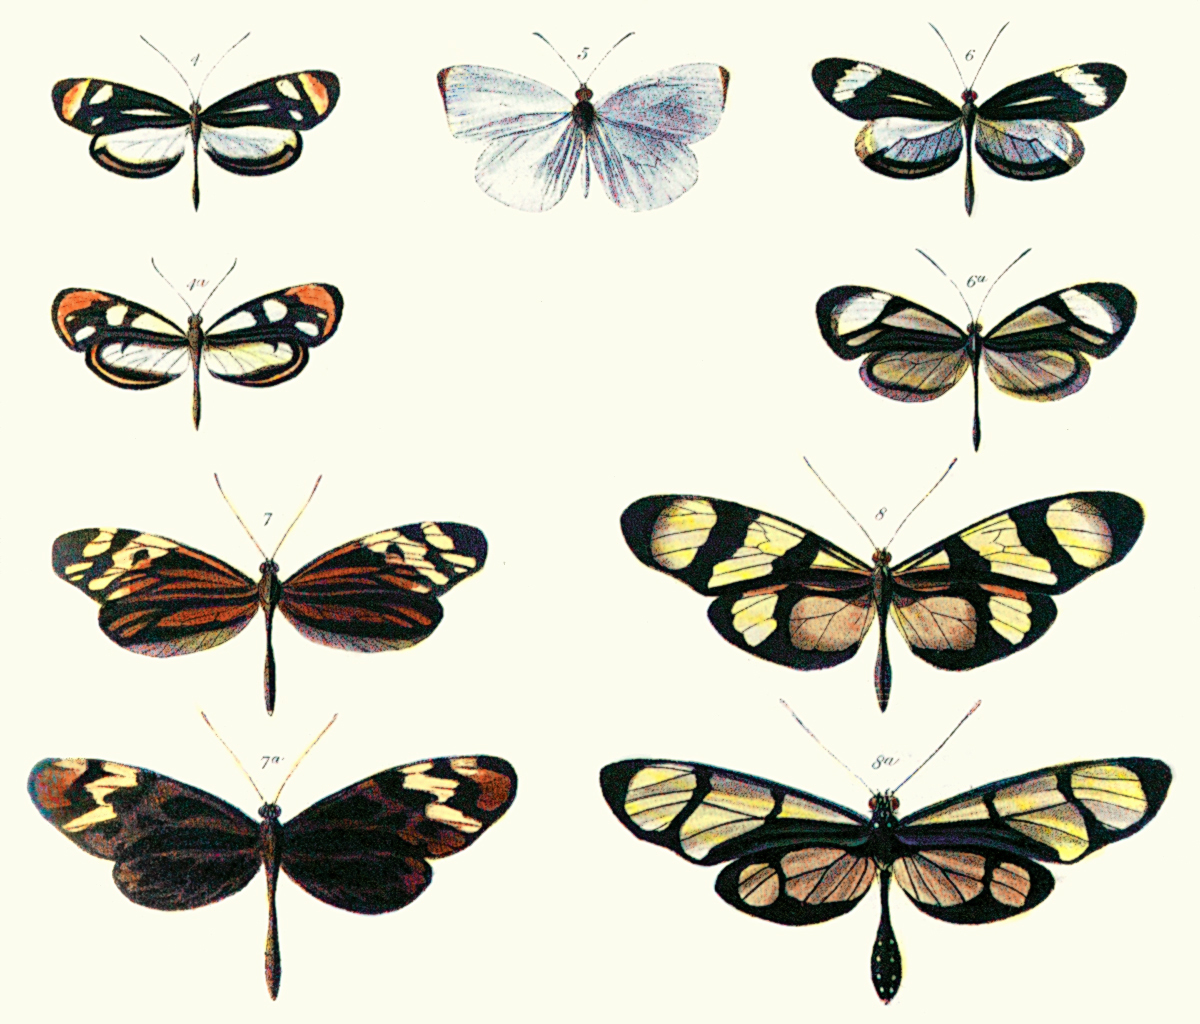
\includegraphics[scale=1]{images/Batesplate_ArM}
	\caption[Plate from Bates (1862) illustrating Batesian mimicry]{Plate from Bates (1862) illustrating Batesian mimicry between Dismorphia species (top row, third row) and various Ithomiini (Nymphalidae) (second row, bottom row). \cite{bates1862}}
	\label{fig:batesian-butterfly}
\end{figure}

\subsection{Definitions of Mimicry}
The following account on the definition of Mimicry is mostly extracted from Wickler's \textit{Mimicry in plants and animals} \cite{wickler1986}. 

According to Wickler the definition of mimicry provided by Bates \cite{bates1862} is quite restricted and is similar to the following

\begin{quote}
\textsl{``resemblance in external appearance, shapes and colors between members of widely distinct families."}
\end{quote}

The following more sophisticated definition was provided at the international Zoological Congress in Washington, 1963,

\begin{quote}
\textsl{``Mimicry is the close resemblance of one organism to another which, because it is unpalatable and conspicuous, is recognized and avoided by some predators at some times."}
\end{quote}

The best known definition of mimicry quoted to the present day, are those given by Wallace and listed in Poulton's \textit{The color of animals, their meaning and use} \cite{poulton1890colours}. The clauses are presented in the following:

\begin{itemize}
	\item \textsl{``that the imitative species occur in the same area and occupy the same station as the imitated".} This increases the probability that a predator will affect both parties concerned. Nevertheless, the model could live in Africa and the mimic in Europe, or vice versa, if the deceptive predator were a migratory bird.
	\item \textsl{``that the imitators are always the more defenseless".} On the contrary, for the case of Mertensian mimicry among coral snakes the more offensive party may occasionally be the mimic.
	\item \textsl{``that the imitators are always less numerous in individuals".} What is meant here is that the deceived animal should encounter the mimic less often than the model. This is true when the deceived animal must learn to recognize model and mimic and when positive and negative experiences carry equal weight. But it is known from various learning experiments that when an animal has learned about warning coloration, negative experiences or punishment stimuli (such as inedibility) can have a stronger and more lasting effect than positive experiences. Accordingly it should be expected that there would be an excess of mimics over models in proportion to the degree of predominance of negative experiences over positive onces. When the deceptive animal possesses an innate reaction to the model the number of mimics can be virtually unlimited. 
	\item \textsl{``that the imitators differ from the bulk of their allies".} The most remarkable cases of mimicry are those where close relatives form divergent models. It is nevertheless highly possible that groups of closely related species may be similar mimics of the same model. Of course, it must always be remembered that species can look very different from their relatives because of adaptations which have nothing to do with mimicry. 
	\item \textsl{``that the imitation, however minute, is external and visible only, never extending to internal characters or to such as do not affect the external appearance."} This criteria, like the previous one is aimed at defining mimicry as a special adaptation. But if one of two closely related species both of which are poisonous and possess similar warning coloration, should secondarily lose its poisonous qualities, it would become a mimic and yet resemble its model in almost all its non-mimetic characters.
\end{itemize}

According to Wickler \cite{wickler1986}, these five requirements, if fulfilled, indeed increase the probability that any given case of mimicry will be correctly diagnosed. But such supplementary clauses cannot be used as a definition of mimicry in general, though this is unfortunately often attempted. 

\section{Mullerian Mimicry}
\label{sec:mullerian-mimicry}
Bates was not able to explain some phenomena of mimicry. Occasionally two inedible unrelated butterfly species are amazingly similar in appearance. An explanation for this was provided by Fritz Muller in 1878. Like Bates, Muller observed and caught butterflies in Brazil. When there are multiple inedible species it is hard for predators to recognize each of them to know which one to consume and which one to avoid. Because of predator's limited memory, all these species still lose their number even after being inedible. So to save this loss, and to prevent more sacrifice of their own kind, inedible species from different family also tend to evolve to have similar appearance. This phenomena is referred to as Mullerian Mimicry in the name of Fritz Muller.

According to Huheey \cite{huheey1988} \textsl{``Mullerian mimicry is normally viewed as a system of mutual warning coloration arising from the convergence of two or more warningly colored species, though two closely related species could also be Mullerian mimics through parallel evolution" \cite{muller1879}.} In Muller's view, predation load on each species are reduced when their warning signals are shared or converged. Naive young predators create the most impact in learning predation as they start their life with no knowledge or experience over the prey species. For cases like these, all unpalatable species should benefit from mutual advertising. If mutation gives opportunity for a single unpalatable prey to resemble a warningly colored species, it is expected to be more likely to survive predation than if the change was in opposite direction. Predators surviving on warningly colored species need to generalize; meaning if similar patterns signal unpalatability, predators recognition rate becomes much higher. Thus, variation in color pattern is tolerated, and mutations leading to even poor resemblance provides some protection. 

It is worth observing the fact that Mullerian mimicry is not deception, as it is to the predator's advantage to be able to recognize all deterrent and noxious species. Preys resemblance does not have to be close enough to cause misidentification on the part of the predator, but merely similar enough to remind it of a bitter past experience with similar prey. As Huheey continues \textsl{``Thus although there is selection for convergence to perhaps the most common, average pattern, or more likely the one associated with the most deterrence (both from the intensity of the traumatic stimuli and the frequency of predators receiving them), the convergence need not be rapid or precise. Indeed, the resemblance among Mullerian mimics is often not close, and the existence of very close mimics raises doubts that the mimicry is Mullerian."}

\begin{figure}[H]
	\centering
	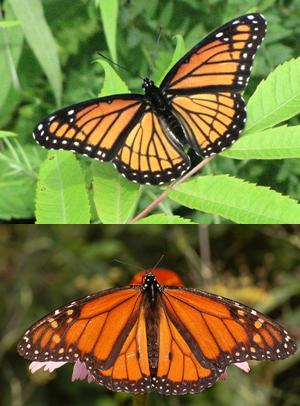
\includegraphics[scale=0.75]{images/BatesMimButter}
	\caption[A very well-known example of mimicry, the viceroy butterfly]{A very well-known example of mimicry is the viceroy butterfly (top) which has a pattern very similar to the unpalatable monarch butterfly (bottom). It was considered for a long time that this is an ideal example of Batesian mimicry. But recently Brower discovered that the viceroy is actually just as noxious as the monarch, making this a case of Mullerian mimicry. \cite{brower1991} Image source: \href{http://en.wikipedia.org/wiki/Mullerian_mimicry}{Wikipedia}}
	\label{fig:mullerian-butterfly}
\end{figure}

\section{Evolutionary Dynamics of Mimicry}
\label{sec:evolutionary-dynamics-of-mimicry}
The dynamics of mimicry has been investigated by Turner \cite{turner1988}, where he states that the evolution of mimicry can be explained best by the process of punctuated equilibrium instead of phyletic gradualism. 

\paragraph{Punctuated Equilibrium}
In evolutionary biology, punctuated equilibrium is the theory which proposes that most sexually reproducing species will remain in an extended state called \textit{stasis} while experiencing little evolutionary change for most of their geological history. When evolution occurs it is localized in rare, rapid events of branching speciation, called cladogenesis. Cladogenesis is the process by which species split into two distinct species, rather than one species gradually transforming into another. Thus, \textsl{``punctuated equilibria is a model for discontinuous tempos of change (in) the process of speciation and the deployment of species in geological time" \cite{gould1977}}. 

\paragraph{Phyletic Gradualism}
In contrast to punctuated equilibrium, phyletic gradualism states that species continue to adapt to new environmental and biological selection pressures over the course of their history, gradually becoming new species. Phyletic gradualism holds that a species population changes gradually; that is there is no clear line of demarcation between an ancestral species and a descendant species unless a splitting (cladogenetic) event occurs or the gradually-changing lineage is divided arbitrarily. During this process, evolution occurs at a smooth, steady and incremental (but not necessarily constant and slow) rate on a geological time scale. 

On this issue Turner states,

\textsl{``According to punctuated equilibrium, therefore, evolution is not more of less both gradual and continual, as has been supposed for most purposes in most post-Darwinian theories. Rather, most morphological change is held to take place within geologically short periods, separated by vastly longer periods of comparative stasis \cite{eldredge1972}. The rapid, large changes all occur during speciation, that is to say during the branching of the evolutionary tree (cladogenesis);" \cite{turner1988}}

\begin{figure}[H]
	\centering
	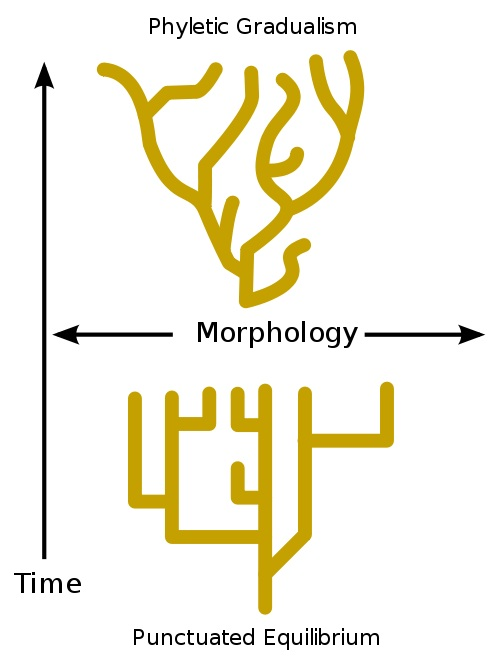
\includegraphics[scale=0.5]{images/Punctuated-equilibrium}
	\caption[Punctuated equilibrium vs. phyletic gradualism]{Punctuated equilibrium, bottom, consists of morphological stability and rare bursts of evolutionary change, while the top explains phyletic gradualism. Image source: \href{http://en.wikipedia.org/wiki/Punctuated_equilibrium}{Wikipedia}}
	\label{fig:punctuated-equilibrium}
\end{figure}

To explain the dynamic evolutionary process of mimicry, Turner came up with a synthetic theory \cite{turner1988}, which was originated by Poulton \cite{poulton1912} and Nicholson \cite{nicholson1927}, termed as the \textbf{two stage model}. This theory states that mimicry normally arises in two steps. A comparative large mutation achieves a good approximate resemblance to the model; it is followed by gradual evolutionary changes that refine the resemblance, in many cases to a high degree of perfection \cite{sheppard1972} \cite{ford1964}. This two-stage theory has been applied for the explanation of Mullerian mimicry as well.

\subsection{Mimicry Ring}
Any theory of Mullerian mimicry has to take into account the phenomenon of the coexistence of multiple mimicry rings. If we examine the local butterfly fauna in any area of the world, we will find that between all the aposomatic (warningly colored and defended) species present there are normally only a limited number of different patterns, normally far smaller than the number of species. Each cluster of species, all sharing a common pattern, is termed as Mullerian mimicry ring. Thus, in the rain forest of South and Central America, most of the long-winged butterflies (ithomiids, danaids, and heliconids) belong to one of only five different rings.

\subsubsection{Formation of Mimicry Rings}
In regards to the formation of mimicry ring Turner \cite{turner1988} has given a theory which takes into account the level of protection of different rings of butterfly species and their difference in phenotypic warning patterns. Different level of variation of these two parameter can give us very different formation of mimicry ring evolution. The cases are considered below.

\begin{itemize}
	\item If we imagine two different rings of similar warning patterns in one single habitat, similar enough that the envelop of protection afforded to one gives some protection to the more extreme variant of the other (in a simplified language, suppose that predators that have sampled species A sometimes avoid the more extreme members of species B because they mistake them as A), then these two species are subject to natural protection for mutual convergence of their patterns. Eventually they will form a rather accurate Mullerian mimicry ring.
	\item By contrast, if the two species have patterns so dissimilar that predators encountering one never imagine that it might be the other (the envelop of protection do not overlap the other species' phenotype distribution), then there is no selection whatever for convergence, and the two patterns will remain distinct indefinitely.
 \item But mutations of color patterns are occurring all the time. Suppose that species B happens to produce a mutation whole pattern falls within the envelop of protection afforded to species A. The mimicry need not be perfect, but if it is good enough, the mutation will have an advantage and will spread. In this way species B may, by a single mutation, become a Mullerian mimic of species A; in other word species B may switch from one Mullerian mimicry ring to another. Clearly, if the mimicry is not perfect, the two patterns will then gradually converge, making the resemblance ever closer. 
\end{itemize}

Like Batesian mimicry, Mullerian mimicry can evolve in two stages: the mutational, one way convergence stage followed by the gradual, mutual convergence stage. It is worth mentioning that in the first stage only the less protected species can adopt the pattern of the better protected species; mutations in the other direction is not favored.

\section{Conclusion}
Mimicry is one of the most fascinating cases of evolutionary biology. This phenomenon has been studied extensively as infinite number of evidence exists in nature. One hundred years after Bates first clearly defined the concept, a review of literature listed 1,500 papers arguing for or against it. And this figure is more than 40 years old as it has been taken from Wilcker \cite{wickler1986}, published in 1968. It is almost impossible to survey all the known examples of Mimicry, and this would in any case be pointless. Then again many examples can be found in Cott's \textit{Adaptive Coloration in Animals} \cite{cott1957}.


%Chapter describing the model
\chapter{Modeling the evolution of mimicry}

\section{Introduction}
%Entire section until past work needs to be revised when the model has been fully described.
The objective of this thesis is to design an agent based artificial life model for simulating the natural process of the evolution of mimicry.

There are mainly two species of agents. These agents have properties and behavior similar to the \textbf{model}, the \textbf{mimic} and the \textbf{predator} in the evolution of mimicry. We represent evolution of pattern for the model and the mimic with the help of Cellular Automata(CA). Cellular Automata can be easily represented by simple rules, which can be expressed as a binary string. The predator will be equipped with a Hopfield network, to be able to have pattern recognition capability. The process of evolution will of course be running at the genetic level. 

The choice of Hopfield Network memory for a predator can be considered appropriate as the number of patterns which can be recognized by this network is inversely proportional to the accuracy of recall. As more patterns are memorized, Hopfiled network tends to make more errors. This behavior will be appropriate for the simulation of Mullerian mimicry. Mullerian mimicry happens because of limited memory of the predators. Because of this limited memory, multiple inedible butterflies seems to converge to a single ring.

The environment will be designed as three dimensional, while the space will be of toroidal nature. This idea has been taken from the Laws and Life project by Peter Grogono \cite{grogono2003}.

\section{Past Work}
Various models of mimicry has been simulated and explored. The model by Turner \cite{turner1996} and the mathematical model of Huheey \cite{huheey1988} tend to focus on the selective pressure on prey brought about by the particular learning abilities of the predator, and employ simple Monte Carlo or mathematical approaches.

Sherratt \cite{sherratt2002} provides an innovative perspective on the evolution of warning signals by considering co-evolving predator and prey populations. The model's predators are deterministic, in that they have a fixed behavioral strategy over their lifetime, and cannot learn from experience. For both cryptic and conspicuous prey, each predator has fixed policy of either attacking or avoiding.

The latest work on modeling evolution of warning signals and mimicry with individual based simulation is done by Frank and Noble. Their initial work \cite{franks2002} seems of focus on putting some conditions of mimetic evolution in an individual based model with multiple species preyed upon by a single abstract predator, where the appearance of each prey species can evolve but their palatability is fixed.

On 2003 \cite{franks2003} another model for the origin of mimicry ring has been proposed by Frank and Noble. Accordingly theory suggests that all Mullerian mimics in an ecosystem should converge into one large ring, while this convergence will be encouraged by presence of Batesian mimics. So an evolutionary simulation to observe the above mentioned phenomenon has been presented in this piece of work.

Frank and Noble continue to test the influence on mimicry ring evolution by Batesian mimics in their work on \cite{franks2004}. Usually mathematical models of mimicry has fixed prey coloration and appearances, which enables a comparison of predation rates to demonstrate the level of protection a mimic might be afforded. In this model prey colorations are free to evolve. This phenomenon is used to examine the effect of Batesian mimicry on Mullerian mimics and mimicry rings. 

\subsection{Models by Frank and Noble}
%Explain more about the first model by Frank and Noble
The first model by Frank and Noble \cite{franks2002} is where ``multiple species are preyed upon by a single abstract predator; the appearance of each prey species can evolve but their palatability is fixed." Each individual had a single gene: a value representing their external appearance or phenotype. The phenotypes are constrained to a ring of values from 1-20 (where 20 and 1 are neighbors). The distance of one phenotype from another represents their levels of similarity. 

A single abstract predator was modeled with a simple reinforcement learning system. The predator's experience of each phenotype was represented by a score, which would be maintained by probability to consume the next prey species depending on similarity or difference in phenotype. 

The existence of mimetic effect were measured with the initial and final distances between prey species' phenotypes. Three experiments were noted. Firstly, with one palatable and one unpalatable species. For this Batesian mimicry was evolved. For the second experiment, with two unpalatable species, Mullerian mimicry was evolved if the two prey species have some initial resemblance. Experiment 3 was carried out with two unpalatable and one palatable species, where the phenotype of the palatable species moved towards that of one of the unpalatable species, which is in other words Batesian Mimicry.

\paragraph{}
The second model by Frank and Noble \cite{franks2003} is based on two working hypothesis:

\begin{enumerate}
	\item \textsl{All of the Mullerian mimics in a given ecosystem should eventually converge into one large ring in order to gain maximum protection.}
	\item \textsl{If the Mullerian mimics do not converge into one large ring, then the presence of Batesian mimics could entice them to do so, by influencing the rings to converge.}
\end{enumerate}

Although there are many mathematical and stochastic models of mimicry in the biological literature, this model gives attention to the evolution of mimicry ring phenomenon from an artificial life perspective.

%\subsubsection{Model Description}
\paragraph{Prey}
Similar to the first model this also contains a population of prey species each having an appearance and palatability level. Different species of prey were each assigned a fixed palatability level on a scale between zero and one (least to most palatable), where 0.5 is neutrally palatable. Palatable species have values greater than 0.5, and unpalatable species have values lower than 0.5. Each prey species has used two genes with values compositely representing their external appearance or phenotype. Both of these genes were constrained to values from 1 - 200. The Euclidean distance of one phenotype from another represented their level of similarity.

\paragraph{Predator}
Similar to Turner's stochastic model \cite{turner_et_al1984},  predators were modeled with a Monte Carlo reinforcement learning system. The predator's experience of each phenotype was represented by an attack probability, which was initialized to ambivalence at 0.5. After eating prey of a particular phenotype, the predator would make a post-attack update of the relevant probability according to the palatability of the prey consumed. The predator would use its experience of different prey appearances to help it decide on whether or not to attack at the next opportunity.

In contrary to the stochastic model \cite{turner_et_al1984},  predators would generalize on the basis of experience. A set of probability formula was used to come up with the current probability to consume a prey species based on its palatability and the previous probability of consumption based on experience using generalization rate and the Euclidean distance between the experienced phenotype and the consumed prey phenotype. 

%Explain the results for the second model by Frank and Noble
\paragraph{Results}
According to the first experiment, which started with 20 unpalatable prey species, hypothesis 1 of a single large mimicry ring was not established. Their was existence of multiple mimicry rings of very different frequency. Second experiment was carried out with some palatable species along with the unpalatable once which was able able to reach conditions of Batesian mimicry also with less mimicry rings, were hypothesis 2 borne out. 

\begin{quote}
\textsl{The presence of Batesian mimics would provide positive selection pressure on mutants and would, therefore, increase the probability that they would evolve an initial resemblance to another unpalatable species. Also, Batesian pressure on mimicry rings has the potential to push one ring into the range of another, helping to bridge a large phenotypic difference between them.}
\end{quote}

\section{FormAL Framework}
The ``FormAL framework" is a collection of ideas and concepts taken from Peter Grogono's FormAL(Formal Artificial Life) project \cite{grogono2003} and are used to build a framework for modeling the evolution of mimicry. The primary goal of the FormAL project was ``\textit{To study the emergence of complexity}". While the principal behind it was ``\textit{not to include a variable in an agent unless the variable is genetically controlled (or, at least, genetically influenced)}". We will see that this principal was not completely established in simulating mimicry as it was not possible to come up with a genetic representation of Hopfield Network which was used as a pattern recognizer for the predator species. 

\subsection{Agents}
In FormAL, an \textbf{Agent} is a simulated organism. It is designed simply, but with the following qualities:

\begin{itemize}
	\item It has behaviors to be able to reproduce itself using genetic information.
	\item Capable of modifying the structure of genome between generations.
	\item Able to interact with other agents.
	\item And also to survive and reproduce in a challenging environment.
\end{itemize}

\subsection{Spatial representation of the environment}
The framework consists of a three dimensional visual environment where agents of the individual based simulation gets complete freedom of movement defined from their genetic representation. 

\paragraph{Space}
The space of the environment is a three-dimensional lattice of discrete points. The coordinate of each point in space is of the form \((x,y,z) \in \Sigma^3\), where \(\Sigma\) be the set \(\{0, 1, ..., S-1\}\). \(S\) is a universal constant being a small positive integer, which in this simulation has been kept at 20 (the value of the \(World Size\) parameter in Table \ref{tab:environment-control-parameters}). 

\paragraph{Time}
Time, being an integer \( (t \geq 0) \), advances in discrete steps in the simulation, where at each step the agents update themselves. 

\paragraph{Cell}
The entire three dimensional toroidal environment is divided in multiple cells. A cell is a three dimensional cubical section of the hyperspace. Accordingly in Table \ref{tab:environment-control-parameters} \(ISize\) is the parameter that controls the number of cells in the environment. The size of a cell is evaluated from the entire world size. And the total number of cell is calculated as \(ISize^3 = 216\).

\begin{table}[H]
\centering
\begin{tabular}{| p{2.2cm} | >{\centering} p{3cm} | p{7.5cm} |}
	\hline
		\textbf{Parameter} & \textbf{Value} & \textbf{Description} \\ \hline
		ISize & 6 & Number of cell in single dimension of the 3-D toroidal cube\\ \hline
		World Size & 20 & Size of a single dimension of the 3-D toroidal cube\\ \hline
		Cell Size & \( World Size / ISize \) & Size of each cell\\ \hline
		Total Number of Cells & \( ISize^3  = 216\) & Total number of cells in the environment\\ 
	\hline
\end{tabular}
\caption{Parameters to control the environment.}
\label{tab:environment-control-parameters}
\end{table}

\begin{table}[H]
\centering
\begin{tabular}{cc}
		\multicolumn{2}{c}{ 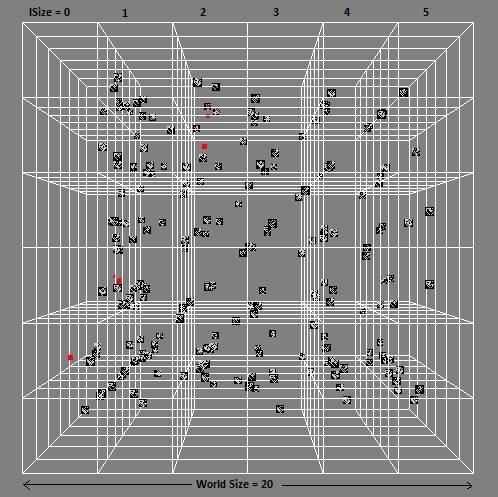
\includegraphics[scale=0.50]{images/cells-front} } \\
		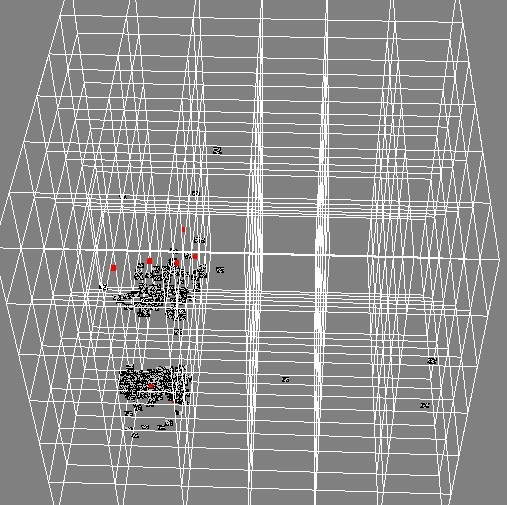
\includegraphics[scale=0.40]{images/cells-top} & 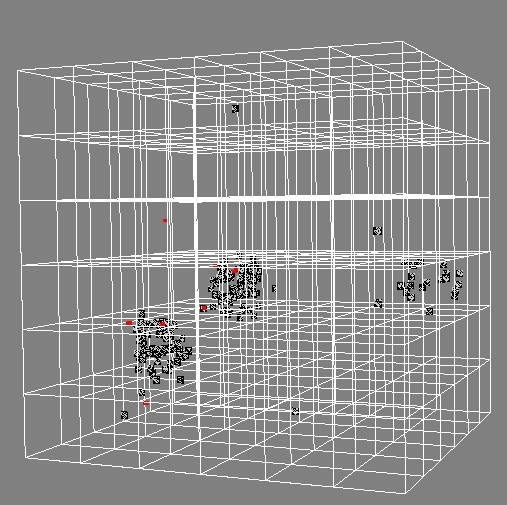
\includegraphics[scale=0.40]{images/cells-side} \\
\end{tabular}
\caption{Three dimensional representation of the environment divided in cells. Presence of different species of agents inside.}
\label{tab:3-d-environment-images}
\end{table}

\subsection{Mobility}
An agents position is calculated once during each step of update in time. The agents \(position\), \(force\), \(acceleration\) and \(velocity\) are all vector components. The \(force\) component is calculated from agent's mobility gene. And it is used to compute agent's \(acceleration\). If the \(force\) and \(velocity\) are both zero, then the agent has no effect in motion. Otherwise, Newton's law is used to obtain the \(acceleration\), which is integrated to obtain the new \(velocity\) and new \(position\).

\begin{algorithm}
	\caption{Algorithm for updating movement of the Agents}
	\label{algo:algorithm-movement-agents}
	\begin{algorithmic}
		\FOR{each step in time}
			\STATE $accelaration \gets ForceFactor * force - Friction * velocity$
			\STATE $velocity \gets DT*accelaration$ \COMMENT{DT is considered as Differential Time Set}
			\STATE $deltaPos \gets DT*velocity$
			\STATE $position \gets position + deltaPos$
		\ENDFOR
	\end{algorithmic}
\end{algorithm}

\begin{table}[H]
\centering
\begin{tabular}{| p{2.2cm} | >{\centering} p{1.3cm} | p{9cm} |}
	\hline
		\textbf{Parameter} & \textbf{Value} & \textbf{Description} \\ \hline
		Force Factor & 40 & A unit vector is multiplied by this amount before being added to the force vector.\\ \hline
		Differential Time Step (DT) & 0.01 & The time step used for first-order integration of the motion equations.\\ \hline
		Friction & 5 & The friction constant used for motion calculations.\\ \hline
		Work Factor & 1 & \( Work done = WF * force * distance \), where \(WF\) is this constant.\\
	\hline
\end{tabular}
\caption{Parameters to control mobility of agents.}
\label{tab:mobility-control-parameters}
\end{table}

Algorithm \ref{algo:algorithm-movement-agents} explains the calculation of mobility of each agent at each time step of the simulation, while Table \ref{tab:mobility-control-parameters} contains the values of the parameters used to apply to this algorithm.

\section{The Prey: Mimics and Models}

\subsection{Pattern representation by Cellular Automata}
Only the significant characteristics which are required for a successful model of mimicry is implemented. As for this simulation we are considering heliconius butterfly, the representation of their wing pattern is with the help of cellular automata. So basically every prey organism will contain a genetic representation of cellular automata with which the predator will identify the prey and store its level of palatability in memory.

%More content needs to be added for cellular automata.
\subsubsection{Cellular Automata}

Cellular automata are computer generated patterns applying very simple rules. First invented by Jon von Neuman and later extended by Stephen Wolfram, this field of study has created a lot of enthusiasm in the evolution of complexity with blocks of simplicity, in this case rules. We choose cellular automata as it can be easily represented with the help of a binary genome and then evolutionary operations on the genomic representation, such as mutation and crossover can easily be applied.

\begin{figure}[H]
	\centering
	
\includegraphics[scale=5]{images/CA_rule30s}
	\caption{Cellular Automata Rule 30.
	Image source: \href{http://en.wikipedia.org/wiki/Cellular_automata}{Wikipedia}}
	\label{fig:cellular-automata-rule-30}
\end{figure}

\begin{table}[H]
	\centering
	\begin{tabular}{| l | c | c | c | c | c | c | c | c |}
	  \hline
	  Current Pattern & 111 & 110 & 101 & 100 & 011 & 010 & 001 & 000 \\ \hline
	  New state of center cell & 0 & 0 & 0 & 1 & 1 & 1 & 1 & 0 \\
	  \hline
	\end{tabular}
	\caption{Cellular Automata Rule}
	\label{tab:cellular-automata-rule}
\end{table}

In generating the pattern of Figure \ref{fig:cellular-automata-rule-30}, the genetic representation would be the 'New state of center cell'. As Figure \ref{fig:cellular-automata-rule-30} is a rule 30 cellular automata, the eight bit binary representation of 30 would be the genetic representation for this pattern. Generation of automata pattern from this binary string can be considered analogous to the complex pathway between the genotype and the phenotype that exists in all living organism.

\subsection{Species diversity}
Franks and Noble have used different models to diversify species. In \cite{franks2002} they have used linear difference in number ``constrained to a 'ring' of values  from 1-20 (where 20 and 1 are neighbors)" to distinguish species diversity. Here the distance of one phenotype from another represents their level of similarity. 

To use CA as prey pattern, its genome is constructed as an 8 bit binary value with a decimal range between 0 to 255. Each of this 256 values have a unique CA pattern associated with it. When storing this pattern in Hopfield memory we take a linear representation of this 2-D pattern, while to consider similarity between two pattern we evaluate the hamming distance between their linear representation. 

With CA based pattern representation, population of prey species with a specific CA pattern can be grouped as one single species. And by restricting inter species reproduction we can control the diversity of patterns. But there is mutation applied when similar species mate with each other, so new species do born out of generations of existing species. So that is why we have two separate mutation rate while reproducing prey species. One being the ``Pattern Mutation Rate" (default values are mentioned in Table \ref{tab:prey-control-parameters}) with which we control mutation of the first 8 bits of the genome while the ``Genome Mutation Rate" is used to control mutation of rest of the 9 bit genome (Table \ref{tab:prey-genome}).

\subsection{Genome}
The Genome of the prey species consists of 17 bits as presented in Table \ref{tab:prey-genome}. The first eight bit is the rule, which is used to generate Cellular Automata pattern. The next two bits are used to represent palatability of the organism explained detail in Section \ref{sec:genetic-palatability-representation}. The next six bits is the force with which mobility of the organism is calculated. The 17th bit is used to evaluate reproduction capability of the organism, depending on which the prey species is either capable or not capable to participate in reproduction.

\begin{table}[H]
\centering
\begin{tabular}{|c|c|c|c|}
	\hline
		\textbf{Pattern(8)} & \textbf{Palatability(2)} & \textbf{Mobility(6)} & \textbf{Reproduction(1)} \\ \hline
		10101101					 	& 							01		 		 & 			110001					&					1						 		 \\ \hline
\end{tabular}
\caption{Distribution and purpose of each gene of the 17 bit prey genome.}
\label{tab:prey-genome}
\end{table}

\subsection{Genetic representation of palatability}
\label{sec:genetic-palatability-representation}
The palatability of each prey species is fixed and has been represented with 2 bit of the genome giving it a range of 0 to 3 with four levels of palatability. The combinations are as follows:

\begin{table}[H]
	\centering
	\begin{tabular}{|c|c|}
		\hline
			\textbf{Gene (Index 8 to 9)} &	\textbf{Palatable} \\ \hline
			00									& True 			\\ \hline
			01									& True 			\\ \hline
			10									& False 		\\ \hline
			11									& False 		\\
		\hline
	\end{tabular}
	\caption{Genetic representation of Palatability}
	\label{tab:genetic-representation-palatability}
\end{table}

This representation in Table \ref{tab:genetic-representation-palatability} is unlike Frank and Noble \cite{franks2003} where palatability level has been used on a scale between zero and one (least to most palatable), where 0.5 is neutrally palatable. 

\subsection{Interaction between other Prey and Predators}
The prey have been defined to have many conglomerate behavior in the environment. Prey interaction with other prey species and with predators make the evolution of mimicry possible. Mobility of prey species and their reproduction capability are two important behaviors which result from interaction. 

\subsubsection{Mobility}
The mobility genes of the prey consist of 6 bits. These six bits are used to calculate the force with which each prey try to move towards any neighborhood cell. The algorithm sorts all neighboring cell descending to the number of prey species. Then it selects the cell which contains the highest number of prey with zero predator. If all the neighboring cells contain predators, then the algorithm sorts the neighboring cells descending on the number of predators and chooses the one which contains the least. Algorithm \ref{algo:algorithm-movement-prey} explains in detail.

\begin{algorithm}[H]
	\caption{Algorithm for updating position of the Prey species}
	\label{algo:algorithm-movement-prey}
	\begin{algorithmic}
		\FOR{each step in time}
			\STATE $forceMagnitude \gets convertToDecimal(genome[10-15])$
			\STATE Get list of neighborhood cells, sorted by population of prey species.
			\STATE From the sorted cell list choose the one with the least number of predators and most number of prey.
			\STATE Move towards the selected cell with $forceMagnitude$ unit of force.
		\ENDFOR
	\end{algorithmic}
\end{algorithm}

\subsubsection{Reproduction}
Every prey species starts reproducing when it reaches the ``Reproductive age limit". If it is capable of reproducing, which is decided based on its 17th bit gene, the prey will randomly select another prey species with similar pattern and palatability from the same cell and mate with it. Now the other prey also needs to be genetically capable of reproduction and needs to reach its age limit. A new genome is created from the existing genome of the two prey by applying single point crossover operation. Mutation is performed separately on the pattern gene and the rest of the genome, with two different rates to control them using the values in Table \ref{tab:prey-control-parameters}. So there is two point mutation for the genome. 

\begin{algorithm}[H]
	\caption{Algorithm for reproduction of the Prey species}
	\label{algo:algorithm-reproduction-prey}
	\begin{algorithmic}
		\FOR{each step in time}
			\STATE $capableToReproduce \gets$ true or false depending on the 17th bit of the genome, and maturity on reproduction age.
			\IF {$capableToReproduce == true$ and $currentCellPopulation > 1$ } 
				\STATE $anotherPrey \gets$ Select random prey from same cell.
				\IF {$anotherPrey$ is alive and $capableToReproduce$ and of similar $pattern$ and $palatability$}
					\STATE Perform genetic cross over and mutation to create new genome.
					\STATE Create new prey with new genome, and release into environment.
					\STATE Record reproduction time for both prey.
				\ENDIF
			\ENDIF
		\ENDFOR
	\end{algorithmic}
\end{algorithm}

\begin{table}[H]
\centering
\begin{tabular}{| p{2.2cm} | >{\centering} p{1.5cm} | p{9cm} |}
	\hline
		\textbf{Parameter} & \textbf{Value} & \textbf{Description} \\ \hline
		Prey Size & 2 to 5 & Size of the prey species in the 3D FormAL  environment.\\ \hline
		Reproduction age limit & 100 & Minimum number of iterations or time steps a prey species need to be present in the simulation to get reproduction capability\\ \hline
		Reproduction interval & 1000 & Number of iterations a prey need to wait before reproducing again.\\ \hline
		Pattern Mutation Rate & 0.05 & Rate of Mutation of the pattern genome.\\ \hline
		Genome Mutation Rate & 0.5 & Rate of mutation of the rest of the genome excluding the pattern gene.\\ \hline
		Demise Age & 2000 & Age at which the prey species will be removed from the environment.\\
	\hline
\end{tabular}
\caption{Parameters to control prey population and visibility.}
\label{tab:prey-control-parameters}
\end{table}

\section{Predator}

Predators in the system are designed to provide selection pressure to \textit{models} and \textit{mimics} for the evolution of mimicry. Similar to prey species, they are agents in the FormAL environment capable of mobility and reproduction. In addition to that these agents are equipped with Hopfield Network Memory to be able to learn and recognize patterns of the prey species. Their mobility and reproduction capability is controlled at the genetic level, but their memory is not, as it was not possible to come up with a genetic representation for Hopfield Network. A set of parameters are defined to control predators' population and learning ability in the environment. Details of the parameters are given in Table \ref{tab:predator-control-parameters}.

\subsection{Learning}
The objective of a predator's interaction with the prey is always to consume it. But based on the species of the prey and depending on its palatability, the predator will either be able to consume it or to throw it back to the environment. At this event the predator needs to learn the pattern with which the prey has been represented. The pattern represents palatability of the prey species, at least to the predator. To store this new pattern into memory, each predator is equipped with a Hopfield Network Memory. Every time a new interaction is made by the predator its memory is initialized with all the existing pattern that has already been encountered and the new one. The learning procedure used for this memory is Hebbian Learning. 

\subsubsection{Hebbian Learning}
\textit{Hebb's postulate of learning} is the oldest and most famous of all learning rules; it is named in honor of the neuropsychologist Donald Hebb(1949). Hebb's book \textit{The Organization of Behavior} (1949) states the following (p.62):

\begin{quote}
\textsl{When an axon of cell A is near enough to excite a cell B and repeatedly or persistently takes part in firing it, some growth process or metabolic changes take place in one or both cells such that A's efficiency as one of the cells firing B is increased.}
\end{quote}

The following \textit{general learning rule} is adopted in neural network studies: \textit{The weight vector} \( \textbf{w}_i = [w_{i1} \> w_{i2} \> ... \> w_{in}]^t \) \textit{increases in proportion to the product of input} \textbf{x} \textit{and learning signal r}. The learning signal r is in general a function of \(\textbf{w}_i,\textbf{x}\), and sometimes of the teacher's signal \(d_i\). Thus we have, 
\begin{equation}
	r = r(\textbf{w}_i,\textbf{x},d_i)
%\label{eq:}
\end{equation}
The increment of the weight vector \(\textbf{w}_i\) produced by the learning step at time t according to the general learning rule is,
\begin{equation}
	\Delta\textbf{w}_i(t)=cr[\textbf{w}_i(t),\textbf{x}(t),d_i(t)]\textbf{x}(t)
%\label{eq:}
\end{equation}
when c is a positive number called the \textit{learning constant} that determines the rate of learning.

For Hebbian learning rule the learning signal is equal simply to the neuron's output. We have
\begin{equation}
	r \overset{\Delta}{=} f(\textbf{w}_i^t \textbf{x})
%\label{eq:}
\end{equation}
The increment \(\Delta\textbf{w}_i\) of the weight vector becomes
\begin{equation}
	\Delta\textbf{w}_i = cf(\textbf{w}_i^t \textbf{x})\textbf{x}
%\label{eq:}
\end{equation}
The single weight \( w_{ij} \) is adapted using the following increment:
\begin{equation}
	\Delta\textit{w}_{ij} = cf(\textbf{w}_i^t \textbf{x})x_j
%\label{eq:}
\end{equation}
This can be written briefly as 
\begin{equation}
	\Delta\textit{w}_{ij} = c o_i x_j, \> \text{for} \> j = 1, 2, ..., n
%\label{eq:}
\end{equation}
The learning rule requires the weight initialization at small random values around \( \textbf{w}_i = \textbf{0}\) prior to learning. The Hebbian learning rule represents a purely feed-forward, unsupervised learning. The rule implements the interpretation of the classic \textit{Hebb's postulate of learning} stated above. 

The rule states that if the cross product of output and input, or correlation term \(o_ix_j\) is positive, this results in an increase of weight \(w_{ij}\); otherwise the weight decreases. It can be seen that the output is strengthened in turn for each input presented. Therefore, frequent input patterns will have most influence at the neuron's weight vector and will eventually produce the largest output.

Training for Hopfield Network used for predator's memory is done by Hebbian Learning. Initially the weights are all set to zero. Using Hebbian rule, the outer product of the input - output vector pairs are calculated for each pattern. As Hopfield is a feedback network, the output of the network is also the input. The outer vector matrix of all the patterns are summed to come up with the final weight matrix. Each component of the weight matrix \(\textbf{W} = \{w_{ij}\}\) is given by:
\begin{equation}
w_{ij} = \sum_{p=1}^{P} s_i(p) t_j(p), i \neq j
%\label{eq:}
\end{equation}
\[
w_{ij} = 0, i = j
\]
where P is the number of patterns. Vectors \textbf{S} and \textbf{T} are respectively, the input and the desired output of the network.

\subsection{Design of Memory with Hopfield Network}

\subsubsection{Hopfield Network}

Algorithm for the Hopfield model is described in the following:

\begin{enumerate}
	\item \textit{Learning.} Let \( \boldsymbol{\xi}_1, \boldsymbol{\xi}_2, ..., \boldsymbol{\xi}_{\mu} \) denote a known set of N-dimensional fundamental memories. Use the outer-product rule (i.e. Hebb's postulate of learning) to compute the synaptic weights of the network as 
	\begin{equation}
		w_{ji} =
			\begin{cases}
				\frac{1}{N} \sum_{\mu=1}^{M}\xi_{\mu,j}\xi_{\mu,i}	& j \neq i \\
				0																										& j = i 
			\end{cases}
	%\label{eq:}
	\end{equation}
	where \(w_{ji}\) is the synaptic weight from neuron \(i\) to neuron \(j\). The elements of the vector \( \boldsymbol{\xi}_\mu \) equal \(\pm 1\) (bipolar). Once they are computed, the synaptic weights are kept fixed.
	
	\item \textit{Initialization.} Let \( \boldsymbol{\xi}_{probe} \) denote an unknown N-dimensional input vector (probe) presented to the network. The algorithm is initialized by setting
	\begin{equation}
		x_j(0) = \xi_{j,probe}, \> j = 1,...,N
	%\label{eq:}
	\end{equation}
	where \( x_j(0) \) is the state of neuron \(j\) at time \(n = 0\) and \( \xi_{j,probe} \) is the \(j\)th element of the probe \( \boldsymbol{\xi}_{probe} \).
	
	\item \textit{Iterate Until Convergence.} Update the elements of state vector \( \boldsymbol{x}(n) \) asynchronously (i.e., randomly and once at a time) according to the rule
	\begin{equation}
		x_j(n+1)=sgn \Bigg(\sum_{i=1}^{N} w_{ji}x_i(n) \Bigg), \> j = 1,2, ..., N
	%\label{eq:}
	\end{equation}
	Repeat the iteration until the state vector \( \boldsymbol{x} \) remains unchanged.
	
	\item \textit{Outputting.} Let \( \boldsymbol{x}_{fixed} \) denote the fixed point (stable state) computed at the end of the step 3, The resulting output vector \( \boldsymbol{y} \) of the network is
	\begin{equation}
		\boldsymbol{y} = \boldsymbol{x}_{fixed}
	\label{eq:}
	\end{equation}
	Step 1 is the storage phase, and steps 2 through 4 constitute the retrieval phase.
\end{enumerate}

\subsubsection{Input to memory}
Each prey contains an evolving cellular automata which is represented by a binary gene. This two dimensional pattern is serialized to be available as a one dimensional binary array, which is taken as input for any predator organism trying to interact with the prey. This binary representation of the pattern gets converted to a bipolar representation. Each input pattern will consist of \(\textit{m} \times \textit{n} = \textit{mn}\) components, each component representing one pixel of the pattern (\textit{m} and \textit{n} representing each dimension). The \textit{m} by \textit{n} pattern configuration will be serialized by putting all row vectors in one single row sequentially.

\subsubsection{Predator attack algorithm}
As soon as a predator reaches its attack age it selects random prey species around its vicinity and starts attacking them. This attack process also involves recognition of prey pattern, which is at the heart of mimicry simulation for this research. Two parameters have been defined to limit predator memorization and recognition process as both of these processes are computationally expensive. The ``Hopfield Minimum Memory Size" (default value in Table \ref{tab:predator-control-parameters}) is the number of memory a predator needs to store before making intelligent decisions about attacking a new prey species. After a predator is born, it start attacking prey without any caution. But after every attack the predator will store its pattern and palatability level inside its memory. As soon as it reaches the minimum memory size, it will start making intelligent decision about attacking the next species. It will try to recognize the pattern and if found palatable, prey will be consumed. Otherwise prey will be thrown back into the environment. If the pattern is not recognized predator will try to consume it and in the process will store its palatability and pattern into memory. 

In this way the predator memory is limited to ``Hopfield Maximum Memory Size". After reaching this memory predator will not store any more new pattern but will try to associate with the existing ones it has already stored. Algorithm \ref{algo:algorithm-attack-prey} and \ref{algo:algorithm-attemptToKill} explains the process in every detail.

\begin{algorithm}
	\caption{Algorithm for attacking Prey species}
	\label{algo:algorithm-attack-prey}
	\begin{algorithmic}
		\FOR{each step in time}
			\IF {Predator has reached Minimum attack age}
				\STATE $preyToAttack \gets$ select random prey species from the same cell.
				\IF {$currentMemorySize < MinimumMemorySize$}
					\STATE $attemptToKill(preyToAttack);$ \COMMENT {Function defined in Algorithm \ref{algo:algorithm-attemptToKill}}
				\ELSE
					\STATE recognize $preyToAttack$ pattern from memory.
					\IF {prey is not recognized or prey is palatable}
						\STATE $attemptToKill(preyToAttack)$
					\ELSE 
						\STATE Prey is recognized as unpalatable, so release it back into environment.
					\ENDIF
				\ENDIF
			\ENDIF
		\ENDFOR
	\end{algorithmic}
\end{algorithm}

\begin{algorithm}
	\caption{$attemptToKill(preyToAttack)$}
	\label{algo:algorithm-attemptToKill}
	\begin{algorithmic}
		\STATE Kill $preyToAttack$.
		\IF {Memory size $< MaxMemorySize$}
			\STATE Associate $preyToAttack$ pattern and palatability and store into memory.
			\STATE Recalculate Hopfield Memory Weights using Hebbian Learning outer product rule.
		\ENDIF
	\end{algorithmic}	
\end{algorithm}

\subsection{Genome}
Each predators has a 5 bit genome as explained in Table \ref{tab:predator-genome}. The first four bit represents its mobility and the magnitude of the force component with which it moves around the environment. The last bit controls reproduction capability of the specific species.

\begin{table}[H]
\centering
\begin{tabular}{|c|c|}
	\hline
		\textbf{Mobility(4)} & \textbf{Reproduction(1)} \\ \hline
				 1101					   &					1						 		\\ \hline
\end{tabular}
\caption{Distribution and purpose of each gene of the 5 bit predator genome.}
\label{tab:predator-genome}
\end{table}

\subsection{Mobility and reproduction capability}
Movement behavior of a predator is calculated from its genome. The first 4 bits of the genome are converted from binary to decimal to determine the magnitude of force at which it will move towards the maximum crowd of prey present within its neighborhood. So magnitude of movement of a predator varies within a range of 0-15 units. If no prey is present in the neighborhood then this force is active in trying to keep predators distributed all over the cells. A predator chooses the neighborhood cell which contains the least number of predators. When the neighborhood contains zero predators, it would select any one of them randomly and move towards that cell.

\begin{algorithm}[h]
	\caption{Algorithm for updating position of the Predator species}
	\label{algo:algorithm-movement-predator}
	\begin{algorithmic}
		\FOR{each step in time}
			\STATE $forceMagnitude \gets convertToDecimal(genome[0-3])$
			\STATE Get list of sorted neighborhood cells. Sorted by population of prey species.
			\STATE From the sorted cell list choose the one with the least number of predators and most number of prey.
			\STATE Move towards the selected cell with $forceMagnitude$ unit of force.
		\ENDFOR
	\end{algorithmic}
\end{algorithm}

\begin{figure}[H]
	\centering
	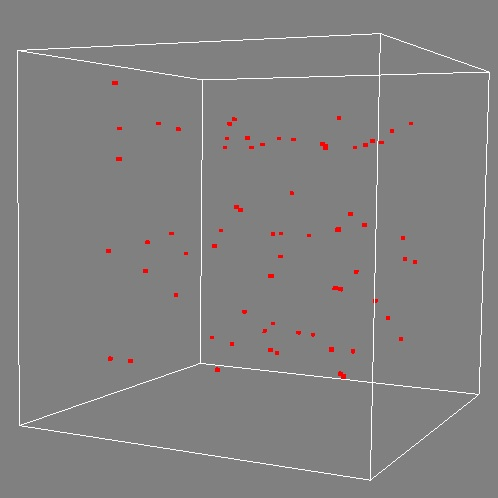
\includegraphics[scale=0.40]{images/predators-40}
	\caption{A population of 40 predators distributed over the environment.}
	\label{fig:predators-40}
\end{figure}

The screen shot in Figure \ref{fig:predators-40} is from the simulation with only 40 predator species. It is presented to show the behavior of predator species in the simulation in absence of any prey species. As it can be observed the predator are distributed all over the cells with a constant mobile behavior to switch to another neighboring cell depending on which ever contains the least number of predator and also most number of prey species. This behavior of predator has been designed to enforce the predatory behavior of this species and also to have increase predator prey interaction in the simulation in terms of one species chasing the other for search of food. 

\subsection{Reproduction process}
The  fifth gene of the predator is used to represent their capability of reproduction.  Depending on its binary value a predator in the simulation will or will not be able to reproduce. The reproduction process for predators is similar to prey species. As the learning capability of predators do not have any genetic representation, only the mobility behavior and reproduction capability takes effect in the reproductive process from one generation to another. 

There are two control parameters that effect the reproduction of predator species. The first is "Reproduction Age Limit". This is the minimum age a predator has to reach before starting to involve itself for reproduction. This parameter has been set to 500 iterations during the result and analysis section of the thesis. The second parameter is "Reproduction Interval" which has been varied in the simulation from 1000 to 3000 iteration depending on the population of palatable prey species. This is a very important parameter for the simulation as it determines the overall predator population and its rate of increment. Depending on this value we can control the rate of predation on prey species, which on the other hand controls the rate of mimetic behavior of the overall prey population.

\begin{algorithm}[H]
	\caption{Algorithm for reproduction of the Predator species}
	\label{algo:algorithm-reproduction-predator}
	\begin{algorithmic}
		\FOR{each step in time}
			\STATE $capableToReproduce \gets$ true or false depending on the 5th bit of the genome, and maturity on reproduction age.
			\IF {$capableToReproduce == true$ and $currentCellPopulationOfPredators > 1$ } 
				\STATE $anotherPredator \gets$ Select random predator from same cell.
				\IF {$anotherPredator$ is alive and $capableToReproduce$ and also reached reproduction maturity age}
					\STATE Perform genetic cross over and mutation to create new genome.
					\STATE Create new predator with new genome and zero memory, and release into environment.
					\STATE Record reproduction time for both predators.
				\ENDIF
			\ENDIF
		\ENDFOR
	\end{algorithmic}
\end{algorithm}

When the above two conditions are met, meaning the predator reaches its age for reproduction and also crosses its age interval, it randomly select another predator residing in the same cell. If this random predator is capable to reproduce depending on its 5th gene, then with a random single point crossover and mutation a new predator species in born which also resides on the same cell and initializes with zero memory configuration. Similarly when the new born predator reaches its maturity of reproductive age and if its capable to reproduce then the process iterates itself. 

\begin{table}[H]
\centering
\begin{tabular}{| p{2.2cm} | >{\centering} p{2.2cm} | p{8cm} |}
	\hline
		\textbf{Parameter} & \textbf{Value} & \textbf{Description} \\ \hline
		Minimum Memory Size & 2 to 6 & Minimum number of patterns stored in memory before predators start making intelligent decisions.\\ \hline
		Maximum Memory Size & 10 & Maximum number of patterns to be stored in memory. Limited to reduce processing time. \\ \hline 
		Hopfield Maximum Iterations & 20 & Maximum number of iterations for Hopfield Network to recognize a pattern. Usually the network reaches a steady state before that. But this restriction is to avoid infinite loop in case the network never reaches a steady state. \\ \hline
		Attack Age & 500 & minimum age a predator needs to reach to be able to attack prey species.  \\ \hline
		Attack Interval & 100 & Interval of time which needs to pass before a predators attacks its next prey. \\ \hline
		Genome Mutation rate & 0.3 & Mutation rate for the 5 bit genome of the predators representing their mobility and pattern recognition capability. \\ \hline
		Reproduction Age Limit & 500 & Minimum age a predator needs to reach before engaging in reproduction.\\ \hline
		Reproduction Interval & 1000 to 3000 & Interval of time a predator needs to pass between two reproduction process.\\ \hline
		Demise Age & 2000 to 7000 & Age at which a predator is considered as dead.\\
	\hline
\end{tabular}
\caption{Parameters to control predator population and pattern recognition capability.}
\label{tab:predator-control-parameters}
\end{table}

\section{Conclusion}

% All the result and analysis
\chapter{The Results}

\begin{quote}
``The most incomprehensible thing about the world is that it is comprehensible." - Albert Einstein
\end{quote}

\section{Introduction}
It is always a challenge to extract and analyze data from an Artificial Life simulation. Data and analysis in this simulation has been concentrated on evaluating whether evolution of mimicry has taken place. This evaluation can be made with the number of different rings that has been created and the size of each of those rings along with the population of palatable and unpalatable species. Also it can be established whether Batesian Mimicry and Mullerian Mimicry has taken effect by analyzing the data set of these populations.

\section{Mimicry Ring Reports}
The mimicry ring reports consists entirely of the population of prey species categorized according to patterns and palatability. Data is stored at every instance of time of the simulation keeping an interval of 10 iterations. As the number of rings that get generated reaches as many as 50 or more, and all the population of ring do not last for the entire simulation, so while storing data we have taken the most populous of the surviving 8 rings to plot. Parameters are mentioned in Table \ref{tab:ring-report-control-parameters}.

\begin{table}[H]
\centering
\begin{tabular}{| p{2cm} | >{\centering} p{2.2cm} | p{8cm} |}
	\hline
		\textbf{Parameter} & \textbf{Value} & \textbf{Description} \\ \hline
		Mimicry Ring Hamming Distance & 10 \% of the Pattern Size & If the Hamming distance between the pattern of the model and the mimic is 10 \% the size of the pattern then they are considered within the same ring.\\ \hline
		Number of Rings to report & 8 & This value is the number of most populous rings that are included in the report.\\
	\hline
\end{tabular}
\caption{Parameters to Mimicry Ring Report.}
\label{tab:ring-report-control-parameters}
\end{table}

\section{Initial configuration with two prey species}
% Put the table here
\begin{table}[H]
\centering
\begin{tabular}{|l|l|c|c|l|c|}
  \hline
   														&\multicolumn{3}{|c|}{Prey configuration} 																	
   														& \multicolumn{2}{|c|}{Predator configuration} \\ \hline
  \multirow{2}{*}{Population} & Rule110 (Palatable) & \parbox[c]{2.1em}{
\includegraphics[scale=0.50]{images/CARule110}} & 108 
  														& \multicolumn{2}{|c|}{\multirow{2}{*}{10}} \\ \cline{2-4}
  					 									& Rule30 (Unpalatable)& \parbox[c]{2.1em}{
\includegraphics[scale=0.50]{images/CARule30}}  & 108 
  					 									& \multicolumn{2}{|c|}{}\\ \hline
  \multirow{2}{*}{Reproduction} & Age Limit & \multicolumn{2}{|c|}{100}  & \multicolumn{2}{|c|}{500} \\ \cline{2-6}
  						 									& Interval  & \multicolumn{2}{|c|}{1000} & \multicolumn{2}{|c|}{1000} \\ \hline
  \multirow{2}{*}{Mutation Rate} & Pattern   & \multicolumn{2}{|c|}{0.05} & \multicolumn{2}{|c|}{\multirow{2}{*}{0.03}} \\ \cline{2-4}
  						 									 & Genome    & \multicolumn{2}{|c|}{0.5}  & \multicolumn{2}{|c|}{} \\ \hline
  Demise Age	 									 & \multicolumn{3}{|c|}{2000}							& \multicolumn{2}{|c|}{2500} \\ \hline
  Minimum Attack Age						 & \multicolumn{3}{|c|}{} 						    & \multicolumn{2}{|c|}{500} \\ \hline
  \multirow{2}{*}{Memory Configuration} & \multicolumn{3}{|c|}{} 					& Minimum & 2 \\ \cline{5-6}
   																			& \multicolumn{3}{|c|}{} 					& Maximum & 10 \\ \hline  
\end{tabular}
\caption{Agent configuration of 2 prey species}
\label{tab:config-table-2-prey}
\end{table}

The set of parameters in Table \ref{tab:config-table-2-prey} were carefully selected to be the initial condition for this run of the simulation. This test has been done with two sets of prey species with very different CA pattern and with opposite palatability and equal population. To control reproduction of the prey species their age limit has been set to 100 iterations into the time the species were alive. And the reproduction interval was set to 1000 iterations.

Pattern mutation rate has been set to a minimal level of 0.05 as by increasing this variable it is possible to increase the size of the number of mimicry rings present in the simulation. The Genome mutation rate controls the rate at which genome of the child prey species will deviate from their parents. As mentioned earlier the genome mutation rate has been separated from the pattern mutation rate to bring more control to the number of mimicry rings generated.

Prey demise age has been kept to 2000 iterations while predator demise age is set to 2500. But later in the following results predator demise age has been increased to 5000 iterations. Predators in this simulation generates selection pressure for the evolution of mimicry. So the longer a predator is present in the simulation it will be making intelligent decisions in term of selecting which prey species to consume and which one to avoid. But with the current rate of demise for predator we were able to create successful mimetic population of prey species as we will see in the analysis in the following results.

Initial population of predator species has been set to 10 which is in accordance with the prey population in the simulation. The reason for such low number of predator is, unlike prey species which are consumed by predators, there is no cause for the predator species to die accept their natural cause of death, that is to reach their demise age. So predator population can explode very easily. That is why their population is controlled in a restrictive manner with the help of high reproduction age limit and reproduction age interval.

The memory configuration size for predators are a very interesting parameter. The minimum memory size is directly associated with the number of prey species with which we initiate the simulation. Otherwise evolution of mimicry is not observed. As mentioned in Table \ref{tab:predator-control-parameters} the minimum memory size is the number of prey species predator would consume before starting to make decisive consumption of prey species. After the initial birth of a predator and when the minimum attack age is crossed, it starts consuming prey species present in its vicinity without making any judgement. At this point its memory size is zero. As long as the minimum memory size is not reached predators will blindly consume prey species and insert their CA pattern and associated palatability into its Hopfield memory bank. No later than the minimum memory size has been reached, predators will start making intelligent decision about consuming its prey species. When catching a prey if its memory tells that it is palatable, it will consume that prey. Otherwise if memory recognizes it to be unpalatable predator will certainly let it go.

Now as we know the behaviour of Hopfield memory, a recognition result will always be achieved depending on the similarity of the patterns stored in memory. So when minimum memory size has been reached the predator will always make a decision based on the similarity of the prey pattern previously captured and the patterns stored in memory.

% Put the image
\begin{figure}[H]
	\centering
	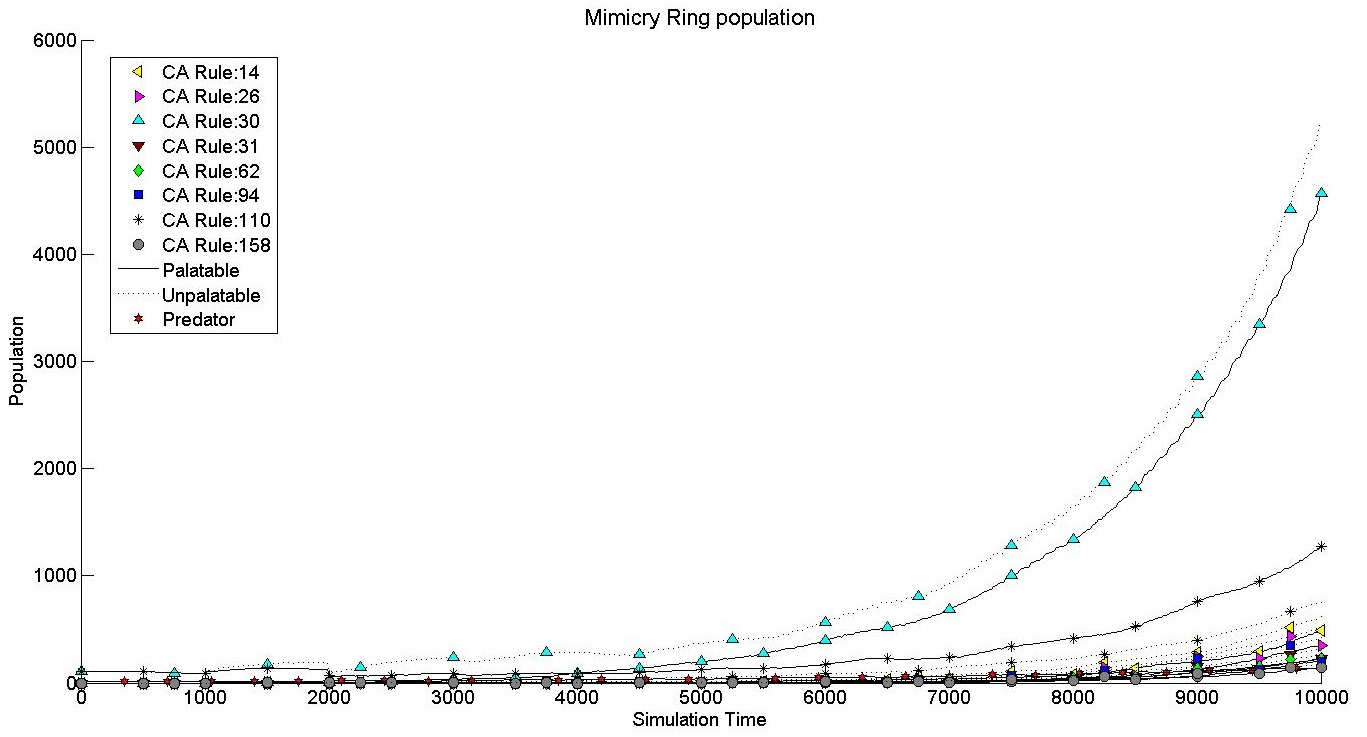
\includegraphics[scale=0.50]{images/simTime10k-2Prey}
	\caption{Population distribution of mimicry rings, initialized with 2 prey species.}
	\label{fig:plot-2-prey}
\end{figure}

The plot in Figure \ref{fig:plot-2-prey} is simulation time verses prey population after running it for over 10000 iterations. With the initial configuration in the above table we can observe that multiple rings of prey population has been created. Two prey species are in a ring if their CA pattern have a hamming distance within 10 bits, parameter mentioned in Table \ref{tab:ring-report-control-parameters}. Population of palatable species has been represented with line curve while population of unpalatable species has been presented with dotted curve. Different signs of squares, triangles and diamonds have been used to distinguish between species of prey population. The simulation was initiated with two prey species having CA rule of 30 and 110 and being palatable and unpalatable consecutively.

By closely observing the graph we could see the population of two species have started dropping at around time 500 when the initial predator population reaches this maturity for consuming prey species. At around time 1000 the prey population starts reproducing as the population increases. At around the same time different other species of prey population gets to be born with mutated CA patterns. Over time the population of CA Rule 110 dominates the population as most predators recognizes it as unpalatable. And similarly a population of CA Rule 110 or within the same ring of palatable species starts rising, while at one point overlaps the population of CA Rule 30 (Time: 5000 approx.) which was initially considered as a set of palatable species.

We can observe from the above results that the evolution of mimicry has taken effect. A population of mimics were successfully able to exceed the population of other prey species the reason being avoidance by predators of prey pattern similar to unpalatable ones. We can conclude that Batesian mimicry has taken effect in the simulation.

The above configuration in Table \ref{tab:config-table-2-prey} is also the most appropriate condition for Mullerian Mimicry. We can observe that a single pattern of unpalatable species dominate the entire population. These effects can be observed in this configuration where we can see the continuous increment of prey and predator population and eventually behaviors of Mullerian mimicry, where all prey species converge to a single ring of CA pattern.

%Put the number of rings picture:
\begin{figure}[H]
	\centering
	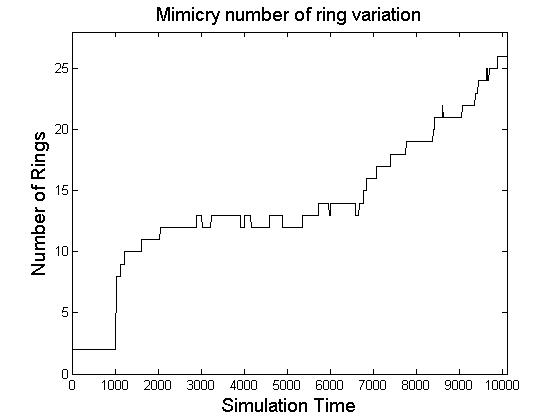
\includegraphics[scale=0.50]{images/ringSize10k-2Prey}
	\caption{Number of mimicry rings, initialized with 2 prey species.}
	\label{fig:ringSize10k-2Prey}
\end{figure}

As it can be observed from Figure \ref{fig:ringSize10k-2Prey} the number of rings in this simulation makes a slow increase from 2 at the initial configuration to 33 rings at the end of 10000 iterations. We can observe that a small change in CA genetic representation can have a very large effect in terms of the phenotype of the pattern with which the prey is represented. For example if we observe the set of pattern genotype with very different phenotype in Table \ref{tab:diff-in-pattern}.

%CARule table
\begin{table}[H]
\centering
\begin{tabular}{|l|c|c|c|}
  \hline
  CA Rule & \(60 \equiv 00111100\) & \(61 \equiv 00111101\) & \(62 \equiv 00111110 \) \\ \hline
  Pattern & \parbox[c]{2.1em}{
\includegraphics[scale=0.50]{images/CARule60}} 
  				& \parbox[c]{2.1em}{
\includegraphics[scale=0.50]{images/CARule61}} 
  				& \parbox[c]{2.1em}{
\includegraphics[scale=0.50]{images/CARule62}}\\
  \hline
\end{tabular}
\caption{Difference in prey pattern genotype and phenotype}
\label{tab:diff-in-pattern}
\end{table}

All the patterns in Table \ref{tab:diff-in-pattern} have a genetic bit difference of 1. So by a single mutation there can be three different set of phenotype for a child organism from its parent. This is largely the reason for the increased number of Rings created in the simulation. Only the 8 most populous rings have presented in the graph above with population verses simulation time.

%Screenshot of the simulation
\begin{figure}[H]
	\centering
	\label{fig:screenshot-simTime7600-2-prey}
	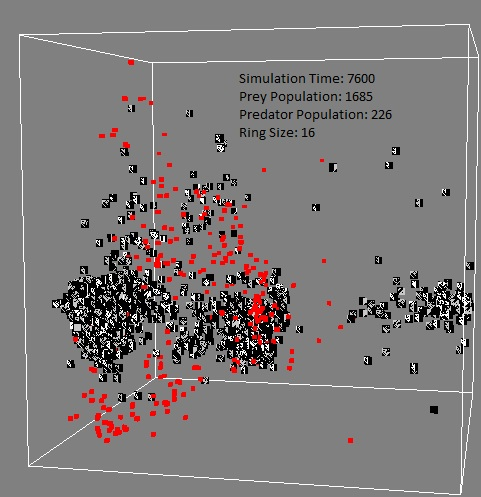
\includegraphics[scale=0.55]{images/simTime7600}
	\caption{Graphical representation of the model, simulation time: 7600.}
\end{figure}

The screen shot in Figure \ref{fig:screenshot-simTime7600-2-prey} is for one instance of time of the simulation. The red agents are predators while the black agents with different textured patterns are the prey species. According to their behavior most of the prey species are flocking together in a group while also being chased by the predators, whose sole purpose is to consume prey species. 

\section{Initial configuration with four prey species}
\begin{table}[H]
\centering
\begin{tabular}{|l|l|c|c|l|c|}
  \hline
   														&\multicolumn{3}{|c|}{Prey configuration} 																	
   														& \multicolumn{2}{|c|}{Predator configuration} \\ \hline
  \multirow{4}{*}{Population} & Rule110 (Unpalatable) & \parbox[c]{2.1em}{
\includegraphics[scale=0.50]{images/CARule110}} 
  																										& 50 & \multicolumn{2}{|c|}{\multirow{4}{*}{10}} \\ \cline{2-4}
  					 									& Rule30 (Palatable)& \parbox[c]{2.1em}{
\includegraphics[scale=0.50]{images/CARule30}}
  					 																					& 50 & \multicolumn{2}{|c|}{}\\ \cline{2-4}
  					 									& Rule55 (Unpalatable)& \parbox[c]{2.1em}{
\includegraphics[scale=0.50]{images/CARule55}}
  					 																					& 50 & \multicolumn{2}{|c|}{}\\ \cline{2-4}
  					 									& Rule190 (Palatable)& \parbox[c]{2.1em}{
\includegraphics[scale=0.50]{images/CARule190}}
  					 																					& 50 & \multicolumn{2}{|c|}{}\\ \hline
  \multirow{2}{*}{Reproduction} & Age Limit & \multicolumn{2}{|c|}{100}  & \multicolumn{2}{|c|}{500} \\ \cline{2-6}
  						 									& Interval  & \multicolumn{2}{|c|}{1000} & \multicolumn{2}{|c|}{1400} \\ \hline
  \multirow{2}{*}{Mutation Rate} & Pattern   & \multicolumn{2}{|c|}{0.05} & \multicolumn{2}{|c|}{\multirow{2}{*}{0.03}} \\ \cline{2-4}
  						 									 & Genome    & \multicolumn{2}{|c|}{0.5}  & \multicolumn{2}{|c|}{} \\ \hline
  Demise Age	 									 & \multicolumn{3}{|c|}{2000}							& \multicolumn{2}{|c|}{2500} \\ \hline
  Minimum Attack Age						 & \multicolumn{3}{|c|}{} 						    & \multicolumn{2}{|c|}{500} \\ \hline
  \multirow{2}{*}{Memory Configuration} & \multicolumn{3}{|c|}{} 					& Minimum & 4 \\ \cline{5-6}
   																			& \multicolumn{3}{|c|}{} 					& Maximum & 10 \\ \hline  
\end{tabular}
\caption{Agent configuration of 4 prey species}
\label{tab:config-table-4-prey}
\end{table}

This run of the simulation has been initialized with four prey species with very different CA pattern configuration. The predator reproduction interval has been increased to 1400, while the minimum memory size has been increased to 4 instead of 2 as the predator is expected to memorize four different species of prey before starting to make intelligent decision about consuming them. 

\begin{figure}[H]
	\centering
	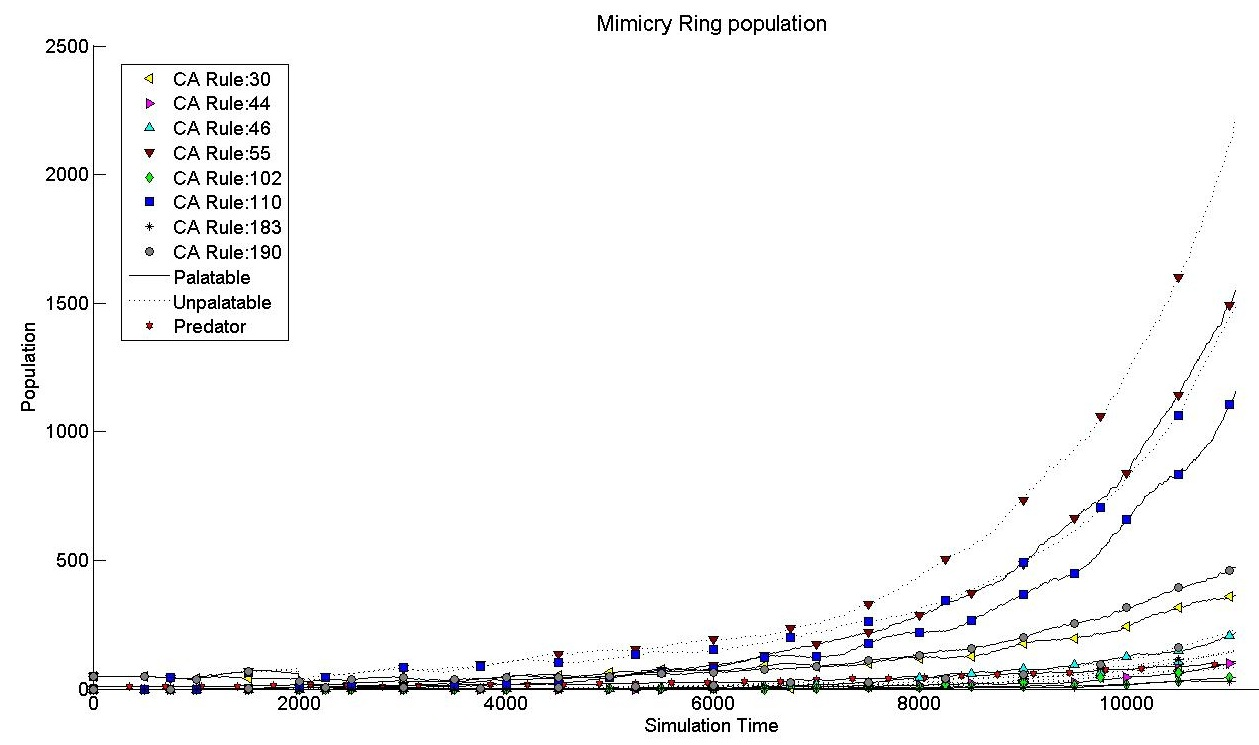
\includegraphics[scale=0.40]{images/simTime10k-4Prey}
	\caption{Population distribution of mimicry rings, initialized with 4 prey species.}
	\label{fig:plot-4-prey}
\end{figure}

By observing the graph in Figure \ref{fig:plot-4-prey} we can see the two rings of unpalatable species which was put at the initial sate of the simulation has dominated after 10000 iterations. CA rule 55 has taken over all other species while CA 110 is following it (represented with dotted curve). Also the palatable prey species with similar patterns to CA rule 55 and 110 are taking full advantage of their deceiving pattern and increasing their population (represented with line curve). The two unpalatable set of patterns CA Rule 90 and 130 are unable to dominate the population. Different other mimicry rings are present in the simulation as we can observe from the graph of number of rings verses simulation time in Figure \ref{fig:ringSize10k-4Prey}, the total number of rings reached somewhere near 33 while each of them has comparatively low representative population. Batesian mimicry is in full effect in this simulated environment.

\begin{figure}[H]
	\centering
	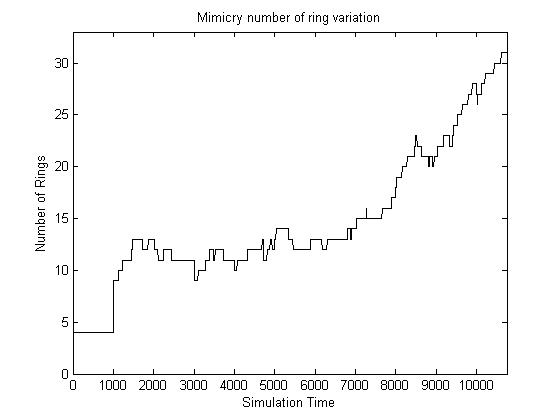
\includegraphics[scale=0.50]{images/ringSize10k-4Prey}
	\caption{Number of mimicry rings, initialized with 4 prey species.}
	\label{fig:ringSize10k-4Prey}
\end{figure}

\begin{figure}[H]
	\centering
	\label{fig:screenshot-simTime11K-4Prey}
	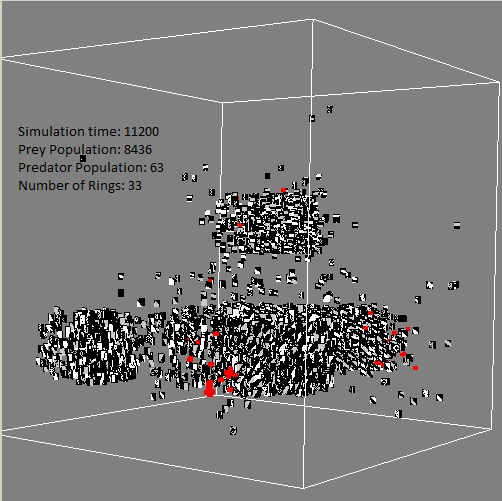
\includegraphics[scale=0.55]{images/simTime11K-4Prey}
	\caption{Graphical representation of the model initialized with 4 prey species, simulation time: 11200.}
\end{figure}

\section{Increased initial population with four prey species}

\begin{table}[H]
\centering
\begin{tabular}{|l|l|c|c|l|c|}
  \hline
   														&\multicolumn{3}{|c|}{Prey configuration} 																	
   														& \multicolumn{2}{|c|}{Predator configuration} \\ \hline
  \multirow{4}{*}{Population} & Rule110 (Palatable) & \parbox[c]{2.1em}{
\includegraphics[scale=0.50]{images/CARule110}} & 150 & \multicolumn{2}{|c|}{\multirow{4}{*}{20}} \\ \cline{2-4}
  					 									& Rule30 (Palatable)& \parbox[c]{2.1em}{
\includegraphics[scale=0.50]{images/CARule30}}  	 & 150 & \multicolumn{2}{|c|}{}\\ \cline{2-4}
  					 									& Rule55 (Unpalatable)& \parbox[c]{2.1em}{
\includegraphics[scale=0.50]{images/CARule55}}  & 150 & \multicolumn{2}{|c|}{}\\ \cline{2-4}
  					 									& Rule190 (Unpalatable)& \parbox[c]{2.1em}{
\includegraphics[scale=0.50]{images/CARule190}}& 150 & \multicolumn{2}{|c|}{}\\ \hline
  \multirow{2}{*}{Reproduction} & Age Limit & \multicolumn{2}{|c|}{100}  & \multicolumn{2}{|c|}{500} \\ \cline{2-6}
  						 									& Interval  & \multicolumn{2}{|c|}{1000} & \multicolumn{2}{|c|}{2500} \\ \hline
  \multirow{2}{*}{Mutation Rate} & Pattern   & \multicolumn{2}{|c|}{0.05} & \multicolumn{2}{|c|}{\multirow{2}{*}{0.03}} \\ \cline{2-4}
  						 									 & Genome    & \multicolumn{2}{|c|}{0.5}  & \multicolumn{2}{|c|}{} \\ \hline
  Demise Age	 									 & \multicolumn{3}{|c|}{2000}							& \multicolumn{2}{|c|}{7000} \\ \hline
  Minimum Attack Age						 & \multicolumn{3}{|c|}{} 						    & \multicolumn{2}{|c|}{500} \\ \hline
  \multirow{2}{*}{Memory Configuration} & \multicolumn{3}{|c|}{} 					& Minimum & 4 \\ \cline{5-6}
   																			& \multicolumn{3}{|c|}{} 					& Maximum & 10 \\ \hline  
\end{tabular}
\caption{Agent configuration of 4 prey species with increased population}
\label{tab:config-table-4-more-prey}
\end{table}

In this run of the simulation some significant parameters have been updated. One is the initial population of prey species. It has been increased from 50 to 150 for each of the prey species, while increasing the overall population from 200 to 600. Secondly the number of predator population has been increased from 20 to 30. Thirdly, Predator demise age has been increased from 2500 to 7000 while their reproduction interval has been increased from 1400 to 2500. Increasing predator demise age can have an interesting effect, as the longer a predator is present in a simulation, the longer it will be making intelligent decision in terms of consuming its prey and there will be increased selection pressure from the entire population of predators. 

\begin{figure}[H]
	\centering
	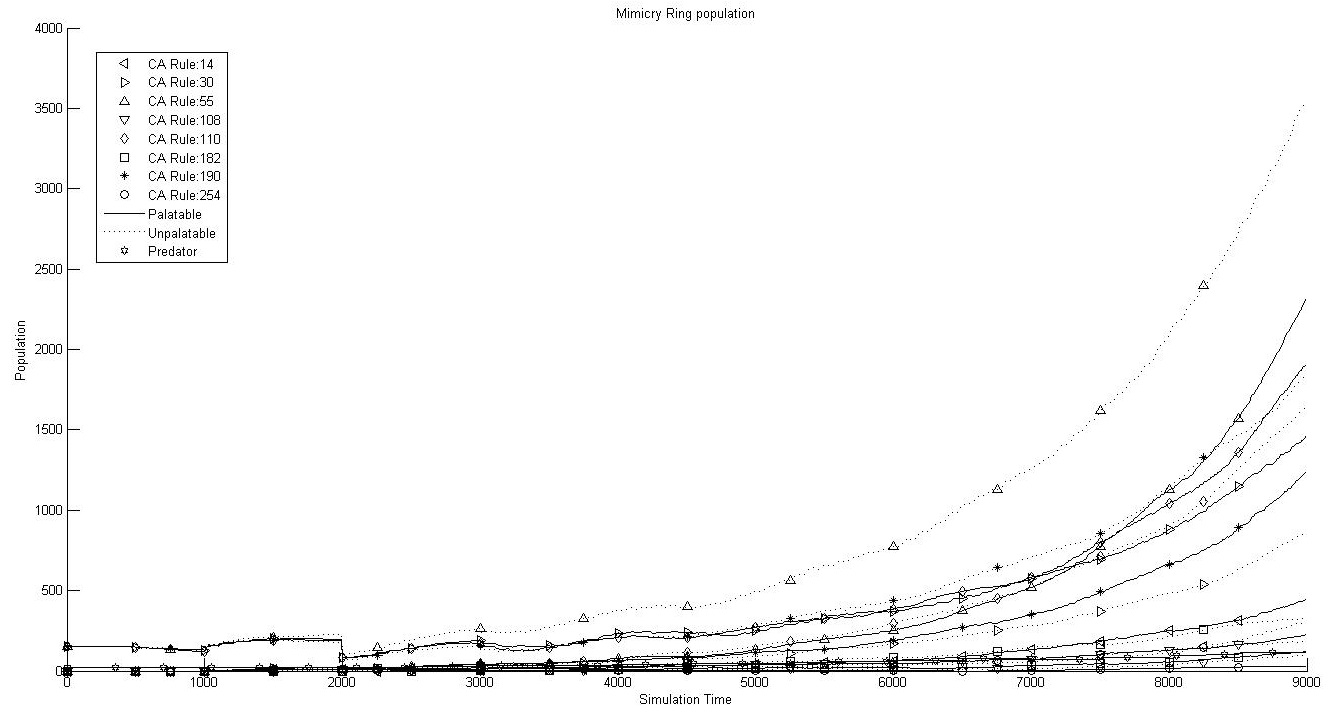
\includegraphics[scale=0.40]{images/simTime9K-4MorePrey}
	\caption{Population distribution of mimicry rings, initialized with 4 prey species with increased population.}
	\label{fig:plot-4-more-prey}
\end{figure}

Some very interesting diversity of rings can be observed in the simulation for updating these parameters. The unpalatable rings and their deceptive counterparts(palatable prey with similar pattern) still have their dominance. We can observe CA Rule 55 and 190 are the highest number of population. Interestingly enough CA Rule 110 which started as a palatable prey species has also taken dominance in the population which is the second highest. Both palatable and unpalatable version of CA Rule 110 are present with equal population density.

\begin{figure}[H]
	\centering
	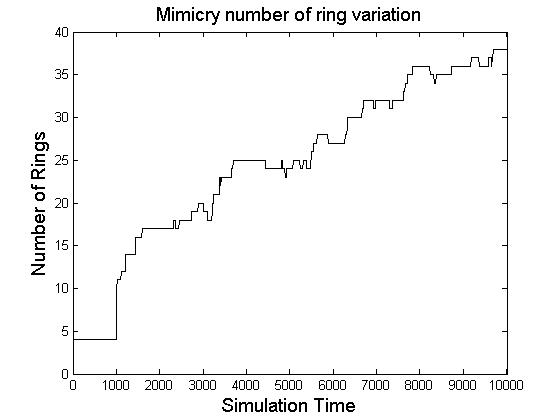
\includegraphics[scale=0.50]{images/ringSize10k-4MorePrey}
	\caption{Number of mimicry rings, initialized with 4 prey species with increased population.}
	\label{fig:ringSize10k-4MorePrey}
\end{figure}

The total number of rings had much increment in this run compared to the previous one. To summarize we can observe increased diversity of prey population and much more interaction between predators and prey.

\section{Initial population with six prey species}
\begin{table}[H]
\centering
\begin{tabular}{|l|l|c|c|l|c|}
  \hline
   														&\multicolumn{3}{|c|}{Prey configuration} 																	
   														& \multicolumn{2}{|c|}{Predator configuration} \\ \hline
  \multirow{6}{*}{Population} & Rule110 (Palatable) & \parbox[c]{2.1em}{
\includegraphics[scale=0.50]{images/CARule110}} 
  																									& 150 & \multicolumn{2}{|c|}{\multirow{6}{*}{30}} \\ \cline{2-4}
  					 									& Rule30  (Unpalatable)& \parbox[c]{2.1em}{
\includegraphics[scale=0.50]{images/CARule30}}  
  					 																				& 150 & \multicolumn{2}{|c|}{}\\ \cline{2-4}
  					 									& Rule55  (Palatable)& \parbox[c]{2.1em}{
\includegraphics[scale=0.50]{images/CARule55}}    
  					 																				& 150 & \multicolumn{2}{|c|}{}\\ \cline{2-4}
  					 									& Rule190 (Unpalatable)& \parbox[c]{2.1em}{
\includegraphics[scale=0.50]{images/CARule190}} 
  					 																				& 150 & \multicolumn{2}{|c|}{}\\ \cline{2-4}
  					 									& Rule57  (Palatable)& \parbox[c]{2.1em}{
\includegraphics[scale=0.50]{images/CARule57}}    
  					 																				& 150 & \multicolumn{2}{|c|}{}\\ \cline{2-4}
  					 									& Rule105 (Unpalatable)& \parbox[c]{2.1em}{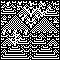
\includegraphics[scale=0.50]{images/CARule105}}& 150 & \multicolumn{2}{|c|}{}\\ \hline
  \multirow{2}{*}{Reproduction} & Age Limit & \multicolumn{2}{|c|}{100}  & \multicolumn{2}{|c|}{500} \\ \cline{2-6}
  						 									& Interval  & \multicolumn{2}{|c|}{1000} & \multicolumn{2}{|c|}{2000} \\ \hline
  \multirow{2}{*}{Mutation Rate} & Pattern   & \multicolumn{2}{|c|}{0.05} & \multicolumn{2}{|c|}{\multirow{2}{*}{0.03}} \\ \cline{2-4}
  						 									 & Genome    & \multicolumn{2}{|c|}{0.5}  & \multicolumn{2}{|c|}{} \\ \hline
  Demise Age	 									 & \multicolumn{3}{|c|}{2000}							& \multicolumn{2}{|c|}{5000} \\ \hline
  Minimum Attack Age						 & \multicolumn{3}{|c|}{} 						    & \multicolumn{2}{|c|}{500} \\ \hline
  \multirow{2}{*}{Memory Configuration} & \multicolumn{3}{|c|}{} 					& Minimum & 6 \\ \cline{5-6}
   																			& \multicolumn{3}{|c|}{} 					& Maximum & 10 \\ \hline  
\end{tabular}
\caption{Agent configuration of 6 prey species.}
\label{tab:config-table-6-prey}
\end{table}

To evaluate the simulation at a more complex level we increase the prey population to 900, consisting of 6 different species with very different pattern configuration. Similarly to increase predator-prey interaction we also increase the number of predator population to 30. Predator reproduction interval has been set comparatively lower in this simulation to 2000 iteration similar to the demise age which is set to 5000. As the initial population of prey species is very high, over time we are expecting even larger number of prey species. If predator population does not increase at similar rate there might be a prey population explosion were predator will have no effect on providing selection pressure for the evolution of mimicry. So that is why predator population control parameter has been set to this level. For memory configuration, the minimum number is set to 6, meaning the predator will have to store 6 different prey pattern configuration before starting to make intelligent decision about consuming them. As previously mention this number is always set in accordance with the initial number of different prey configuration. 

\begin{figure}[H]
	\centering
	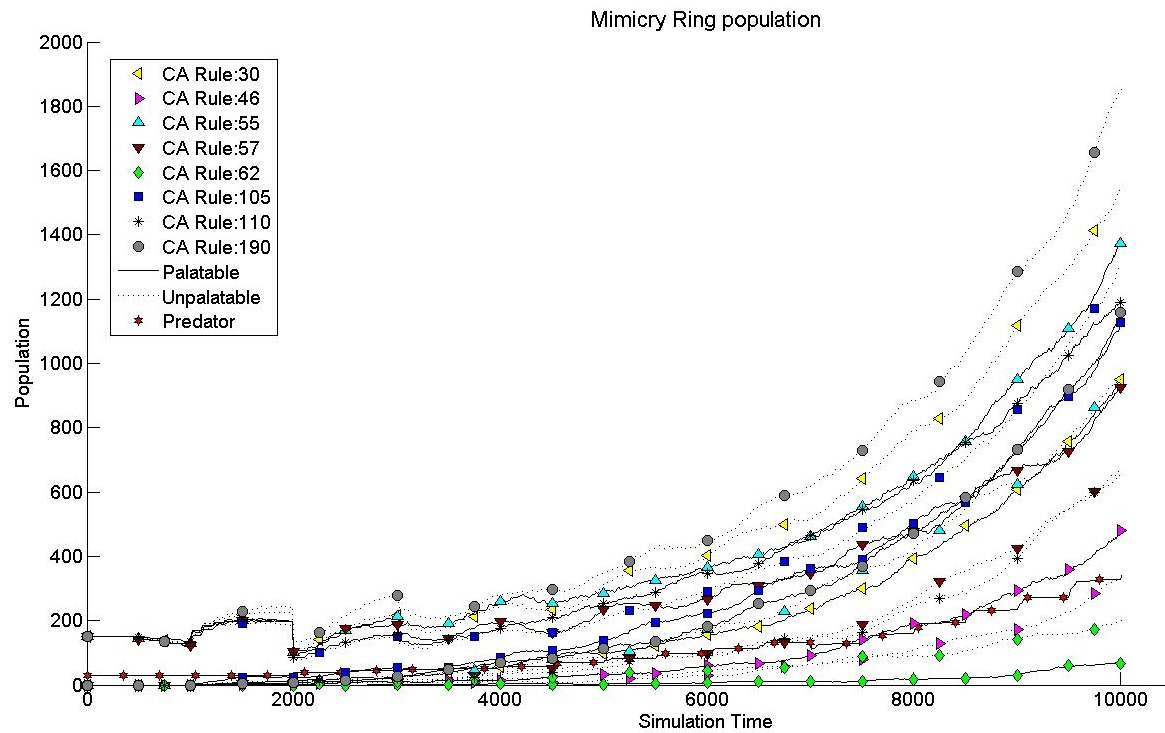
\includegraphics[scale=0.40]{images/simTime10k-6Prey}
	\caption{Population distribution of mimicry rings, initialized with 6 prey species.}
	\label{fig:plot-6-prey}
\end{figure}

With the above set of parameters we can receive the plot of Figure \ref{fig:plot-6-prey}. 

\begin{figure}[H]
	\centering
	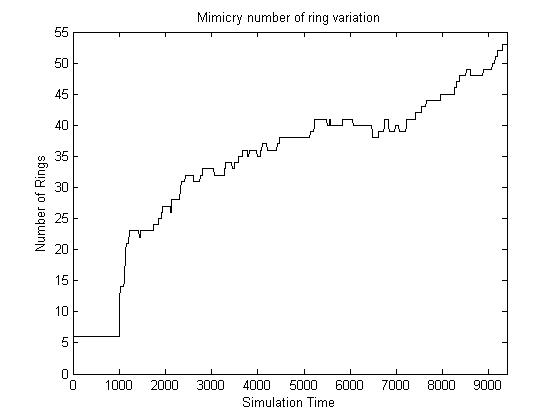
\includegraphics[scale=0.50]{images/ringSize10k-6Prey}
	\caption{Number of mimicry rings, initialized with 6 prey species.}
	\label{fig:ringSize10k-6-Prey}
\end{figure}

\section{Initial configuration with only unpalatable species}
\label{sec:init-conf-only-unp}
\begin{table}[H]
\centering
\begin{tabular}{|l|l|c|c|l|c|}
  \hline
   														&\multicolumn{3}{|c|}{Prey configuration} 																	
   														& \multicolumn{2}{|c|}{Predator configuration} \\ \hline
  \multirow{4}{*}{Population} & Rule110 (Unpalatable) & \parbox[c]{2.1em}{
\includegraphics[scale=0.50]{images/CARule110}} 
  																									& 150 & \multicolumn{2}{|c|}{\multirow{4}{*}{30}} \\ \cline{2-4}
  					 									& Rule30  (Unpalatable)& \parbox[c]{2.1em}{
\includegraphics[scale=0.50]{images/CARule30}}  
  					 																				& 150 & \multicolumn{2}{|c|}{}\\ \cline{2-4}
  					 									& Rule55  (Unpalatable)& \parbox[c]{2.1em}{
\includegraphics[scale=0.50]{images/CARule55}}    
  					 																				& 150 & \multicolumn{2}{|c|}{}\\ \cline{2-4}
  					 									& Rule190 (Unpalatable)& \parbox[c]{2.1em}{
\includegraphics[scale=0.50]{images/CARule190}}& 150 & \multicolumn{2}{|c|}{}\\ \hline
  \multirow{2}{*}{Reproduction} & Age Limit & \multicolumn{2}{|c|}{100}  & \multicolumn{2}{|c|}{500} \\ \cline{2-6}
  						 									& Interval  & \multicolumn{2}{|c|}{1000} & \multicolumn{2}{|c|}{2000} \\ \hline
  \multirow{2}{*}{Mutation Rate} & Pattern   & \multicolumn{2}{|c|}{0.05} & \multicolumn{2}{|c|}{\multirow{2}{*}{0.03}} \\ \cline{2-4}
  						 									 & Genome    & \multicolumn{2}{|c|}{0.5}  & \multicolumn{2}{|c|}{} \\ \hline
  Demise Age	 									 & \multicolumn{3}{|c|}{2000}							& \multicolumn{2}{|c|}{5000} \\ \hline
  Minimum Attack Age						 & \multicolumn{3}{|c|}{} 						    & \multicolumn{2}{|c|}{500} \\ \hline
  \multirow{2}{*}{Memory Configuration} & \multicolumn{3}{|c|}{} 					& Minimum & 4 \\ \cline{5-6}
   																			& \multicolumn{3}{|c|}{} 					& Maximum & 10 \\ \hline  
\end{tabular}
\caption{Agent configuration of 4 prey species all unpalatable.}
\label{tab:config-table-4-prey-unpalatable}
\end{table}

To further observe the effects of mimicry ring we initialize the simulation with four unpalatable population of prey species. As explained earlier the minimum memory configuration is set to 4 as the initial population of prey has four different species. 

\begin{figure}[H]
	\centering
	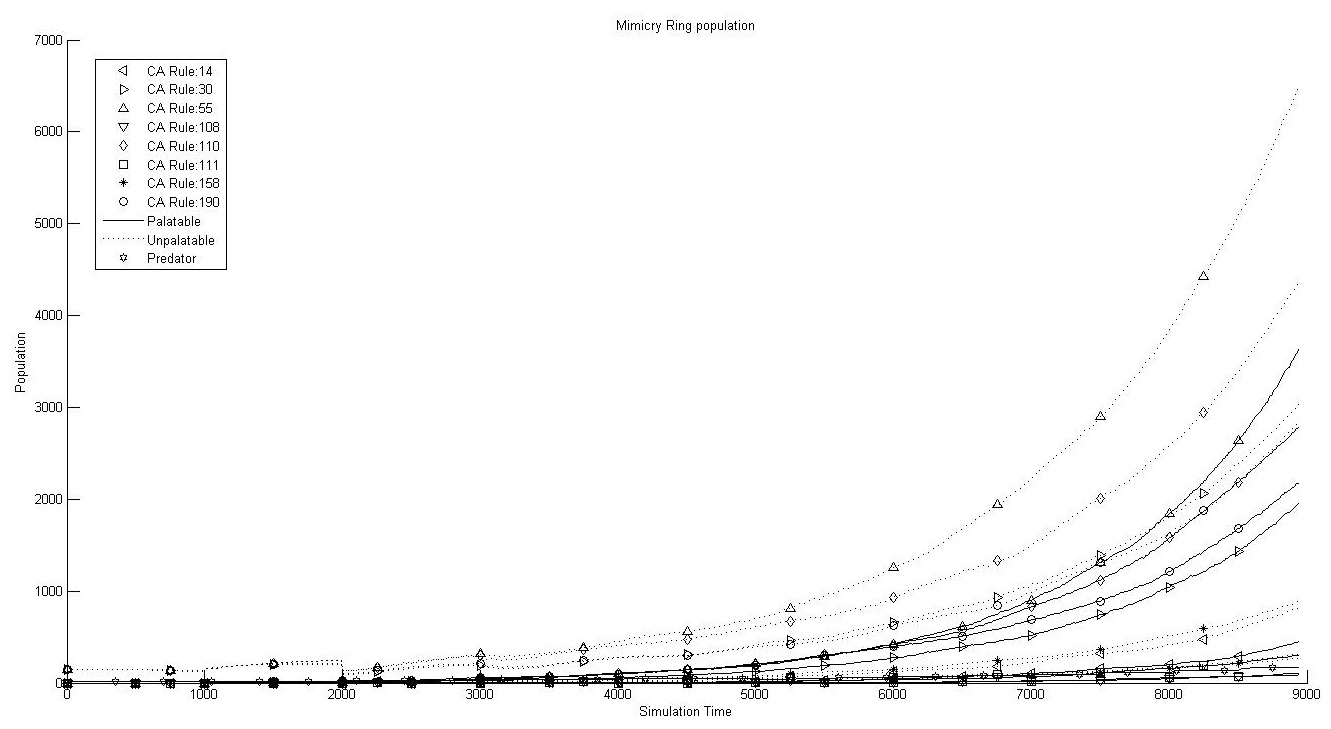
\includegraphics[scale=0.40]{images/simTime-9k-4Prey-unp}
	\caption{Population distribution of mimicry rings, initialized with 4 prey species all unpalatable.}
	\label{fig:plot-4-prey-unp}
\end{figure}

The results according to Figure \ref{fig:plot-4-prey-unp} are expected as it can be observed the population of unpalatable species has prevailed. After nearly 9000 iterations we can see unpalatable species CA rule 55 has prevailed with the most population. Its palatable counter part is following this population. Unpalatable CA Rule 110 and its palatable counter part are also following the above. Similarly the other two species are increasing its population with dominance where the palatable population of deceivers are following them. 

\begin{figure}[H]
	\centering
	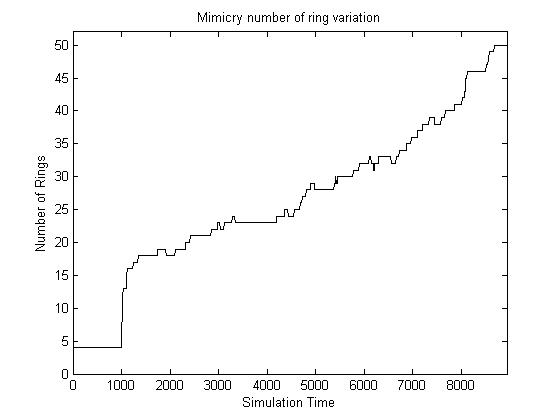
\includegraphics[scale=0.50]{images/ringSize9k-4Prey-unp}
	\caption{Number of mimicry rings, initialized with 4 prey species all unpalatable.}
	\label{fig:ringSize10k-4-Prey-unp}
\end{figure}

\section{Initial configuration with only palatable species}
\label{sec:init-only-palatable-species}

\begin{table}[H]
\centering
\begin{tabular}{|l|l|c|c|l|c|}
  \hline
   														&\multicolumn{3}{|c|}{Prey configuration} 																	
   														& \multicolumn{2}{|c|}{Predator configuration} \\ \hline
  \multirow{4}{*}{Population} & Rule110 (Palatable) & \parbox[c]{2.1em}{
\includegraphics[scale=0.50]{images/CARule110}} 
  																									& 150 & \multicolumn{2}{|c|}{\multirow{4}{*}{30}} \\ \cline{2-4}
  					 									& Rule30  (Palatable)& \parbox[c]{2.1em}{
\includegraphics[scale=0.50]{images/CARule30}}  
  					 																				& 150 & \multicolumn{2}{|c|}{}\\ \cline{2-4}
  					 									& Rule55  (Palatable)& \parbox[c]{2.1em}{
\includegraphics[scale=0.50]{images/CARule55}}    
  					 																				& 150 & \multicolumn{2}{|c|}{}\\ \cline{2-4}
  					 									& Rule190 (Palatable)& \parbox[c]{2.1em}{
\includegraphics[scale=0.50]{images/CARule190}}& 150 & \multicolumn{2}{|c|}{}\\ \hline
  \multirow{2}{*}{Reproduction} & Age Limit & \multicolumn{2}{|c|}{100}  & \multicolumn{2}{|c|}{500} \\ \cline{2-6}
  						 									& Interval  & \multicolumn{2}{|c|}{1000} & \multicolumn{2}{|c|}{2000} \\ \hline
  \multirow{2}{*}{Mutation Rate} & Pattern   & \multicolumn{2}{|c|}{0.05} & \multicolumn{2}{|c|}{\multirow{2}{*}{0.03}} \\ \cline{2-4}
  						 									 & Genome    & \multicolumn{2}{|c|}{0.5}  & \multicolumn{2}{|c|}{} \\ \hline
  Demise Age	 									 & \multicolumn{3}{|c|}{2000}							& \multicolumn{2}{|c|}{5000} \\ \hline
  Minimum Attack Age						 & \multicolumn{3}{|c|}{} 						    & \multicolumn{2}{|c|}{500} \\ \hline
  \multirow{2}{*}{Memory Configuration} & \multicolumn{3}{|c|}{} 					& Minimum & 4 \\ \cline{5-6}
   																			& \multicolumn{3}{|c|}{} 					& Maximum & 10 \\ \hline  
\end{tabular}
\caption{Agent configuration of 4 prey species all palatable.}
\label{tab:config-table-4-prey-palatable}
\end{table}

The parameters for this simulation has been set exactly the same as in Table \ref{tab:config-table-4-prey-unpalatable} except all the species are palatable at this point. All predator configuration has also been set to exactly same as before.

\begin{figure}[H]
	\centering
	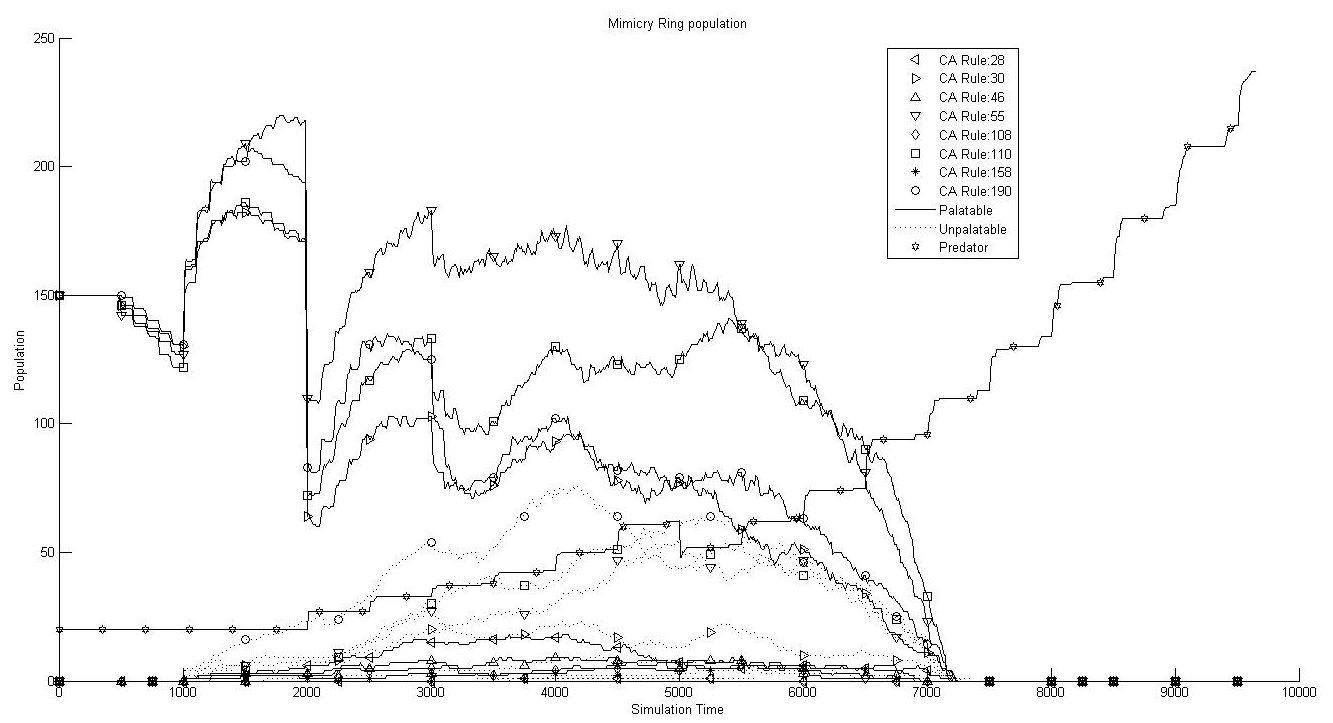
\includegraphics[scale=0.40]{images/simTime-9k-4Prey-p}
	\caption{Population distribution of mimicry rings, initialized with 4 prey species all palatable.}
	\label{fig:plot-4-prey-p}
\end{figure}

The results for the configuration in Table \ref{tab:config-table-4-prey-palatable} can be observed in Figure \ref{fig:plot-4-prey-p} where all population of prey species have reached its demise at nearly 7000 iterations. By analyzing details we can see, around simulation time 500 all population of species comes to a steady downfall as at this point initial predator species reaches its age for consumption. Around simulation time 1000 all population of prey species start increasing steadily because they reach their maturity level of reproduction. At iteration time 2000 a sudden drop of prey population because the initial population of prey have reached its demise age at this point. By this time the population of unpalatable species deceiving the palatable ones start increasing, and slowly around time 7000 and onwards the entire population of prey comes to its demise. Predator population, from the beginning of the simulation has taken a very dominant effect. As all the species are palatable, predator's consumption and reproduction rate is extremely high and it keeps increasing in a geometric rate.

\begin{figure}[H]
	\centering
	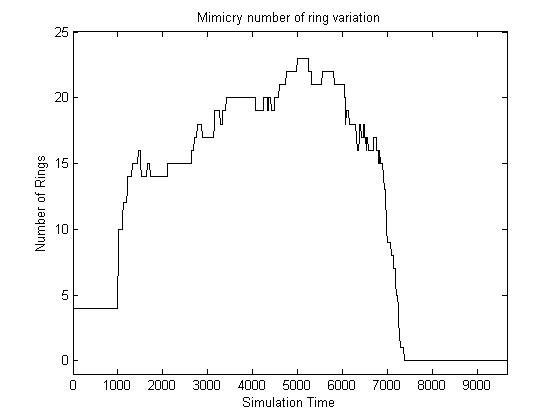
\includegraphics[scale=0.50]{images/ringSize8k-4Prey-p}
	\caption{Number of mimicry rings, initialized with 4 prey species all palatable.}
	\label{fig:ringSize8k-4-Prey-p}
\end{figure}

Observation of mimicry rings also tell us about the results we have seen in the plot of Figure \ref{fig:plot-4-prey-p}. The number of rings keep increasing but comes to a sudden drop around simulation time 7000 it goes to zero.

\section{Initial configuration with single prey species}
Until now all experiments have been initialized with multiple prey species. The following set of experiments have been done with only a single prey species, for both cases of palatable and unpalatable.

\subsection{Unpalatable}
\label{subsec:single-prey-unpalatable}

\begin{table}[H]
\centering
\begin{tabular}{|l|l|c|c|l|c|}
  \hline
   														&\multicolumn{3}{|c|}{Prey configuration} 																	
   														& \multicolumn{2}{|c|}{Predator configuration} \\ \hline
  Population 									& Rule30 (Unpalatable) & \parbox[c]{2.1em}{
\includegraphics[scale=0.50]{images/CARule30}} 
  																									& 216 & \multicolumn{2}{|c|}{10} \\ \hline
  \multirow{2}{*}{Reproduction} & Age Limit & \multicolumn{2}{|c|}{100}  & \multicolumn{2}{|c|}{500} \\ \cline{2-6}
  						 									& Interval  & \multicolumn{2}{|c|}{1000} & \multicolumn{2}{|c|}{2500} \\ \hline
  \multirow{2}{*}{Mutation Rate} & Pattern   & \multicolumn{2}{|c|}{0.05} & \multicolumn{2}{|c|}{\multirow{2}{*}{0.03}} \\ \cline{2-4}
  						 									 & Genome    & \multicolumn{2}{|c|}{0.5}  & \multicolumn{2}{|c|}{} \\ \hline
  Demise Age	 									 & \multicolumn{3}{|c|}{2000}							& \multicolumn{2}{|c|}{7000} \\ \hline
  Minimum Attack Age						 & \multicolumn{3}{|c|}{} 						    & \multicolumn{2}{|c|}{500} \\ \hline
  \multirow{2}{*}{Memory Configuration} & \multicolumn{3}{|c|}{} 					& Minimum & 2 \\ \cline{5-6}
   																			& \multicolumn{3}{|c|}{} 					& Maximum & 10 \\ \hline  
\end{tabular}
\caption{Agent configuration of 1 prey species unpalatable.}
\label{tab:config-table-1-prey-unpalatable}
\end{table}

This configuration has only one unpalatable species, one in each of the 216 cells, equally distributed all over the environment. Also have a set of 10 predators. Their minimum memory configuration has been set to 2 as any value below 2 will not help the Hopfield Network Memory to differentiate between two patterns.

\begin{figure}[H]
	\centering
	\includegraphics[scale=0.40]{images/simTime8k-1-unp}
	\caption{Population distribution of mimicry rings, initialized with 1 prey species unpalatable.}
	\label{fig:plot-1-prey-unp}
\end{figure}

From Figure \ref{fig:plot-1-prey-unp}, it can be observed, the initial set of unpalatable species is dominant as expected. And the palatable population mimicking that set is following it. Also a bunch of other rings with majority of unpalatable species have been created. Mainly because the initial population started with a bunch of unpalatable species, so their evolving generations have similar behavior as well.

\begin{figure}[H]
	\centering
	\includegraphics[scale=0.50]{images/ringSize8k-1Prey-unp}
	\caption{Number of mimicry rings, initialized with 1 prey species unpalatable.}
	\label{fig:ringSize8k-1-Prey-unp}
\end{figure}

\subsection{Palatable}
\begin{table}[H]
\centering
\begin{tabular}{|l|l|c|c|l|c|}
  \hline
   														&\multicolumn{3}{|c|}{Prey configuration} 																	
   														& \multicolumn{2}{|c|}{Predator configuration} \\ \hline
  Population 									& Rule30 (Palatable) & \parbox[c]{2.1em}{\includegraphics[scale=0.50]{images/CARule30}} 
  																									& 216 & \multicolumn{2}{|c|}{8} \\ \hline
  \multirow{2}{*}{Reproduction} & Age Limit & \multicolumn{2}{|c|}{100}  & \multicolumn{2}{|c|}{500} \\ \cline{2-6}
  						 									& Interval  & \multicolumn{2}{|c|}{1000} & \multicolumn{2}{|c|}{2500} \\ \hline
  \multirow{2}{*}{Mutation Rate} & Pattern   & \multicolumn{2}{|c|}{0.05} & \multicolumn{2}{|c|}{\multirow{2}{*}{0.03}} \\ \cline{2-4}
  						 									 & Genome    & \multicolumn{2}{|c|}{0.5}  & \multicolumn{2}{|c|}{} \\ \hline
  Demise Age	 									 & \multicolumn{3}{|c|}{2000}							& \multicolumn{2}{|c|}{7000} \\ \hline
  Minimum Attack Age						 & \multicolumn{3}{|c|}{} 						    & \multicolumn{2}{|c|}{500} \\ \hline
  \multirow{2}{*}{Memory Configuration} & \multicolumn{3}{|c|}{} 					& Minimum & 2 \\ \cline{5-6}
   																			& \multicolumn{3}{|c|}{} 					& Maximum & 10 \\ \hline  
\end{tabular}
\caption{Agent configuration of 1 prey species palatable.}
\label{tab:config-table-1-prey-palatable}
\end{table}

This configuration is set exactly as according to Section \ref{subsec:single-prey-unpalatable} but with a single set of palatable species. The population of predators have been reduced from 10 to 8 to avoid elimination of all prey species as it happened in case of Section \ref{sec:init-only-palatable-species}.

\begin{figure}[H]
	\centering
	\includegraphics[scale=0.40]{images/simTime9k-1-p}
	\caption{Population distribution of mimicry rings, initialized with 1 prey species palatable.}
	\label{fig:plot-1-prey-p}
\end{figure}

From the initial palatable population we see a bunch of palatable rings created. Major difference from Section \ref{subsec:single-prey-unpalatable} is the total number of prey population created. For the unpalatable species section, total population reaches above 12 thousand. But for palatable species total population reaches nearly above 5000 prey species.

\begin{figure}[H]
	\centering
	\includegraphics[scale=0.50]{images/ringSize8k-1Prey-p}
	\caption{Number of mimicry rings, initialized with 1 palatable prey species.}
	\label{fig:ringSize8k-1-Prey-p}
\end{figure}

\section{Analysis of Batesian Mimicry}
For all possible initial conditions, Batesian mimicry has taken effect. It can be observed that for every ring of unpalatable species there is an existence of the palatable ring racing to reach the population count of its unpalatable counterpart. Also when the initial population starts with a set of only palatable species we can observe that the total population vanishes within very short period of time (section \ref{sec:init-only-palatable-species}). This effect can be explained with the fact that the palatable population does not have any models to mimic, and it reaches extinction. So from the analysis it can be concluded that the model under discussion has successfully simulated the evolution of Batesian mimicry.

\section{Analysis of Mullerian Mimicry}
Effects of Mullerian mimicry can be observed best for the experiment in section \ref{sec:init-conf-only-unp}. In this experiment we initialize the model with 4 rings of unpalatable species with no palatable ones and after nearly 10K iterations we can observe that all of the initial unpalatable rings have survived with dominance. So we can be conclude that our results match with the one from Frank and Noble (section \ref{subsec:models-by-frank-and-noble}), that multiple Mullerian mimics do not converge into one large ring.

\section{Conclusion}
Analysis of the results tell us that we have successfully been able to simulate the evolution of mimicry. In addition to that, this model provides a more accurate simulation of the fascinating natural process of mimicry rings. Not only does this model simulates mimicry with the initialized population but also it provides possibility of creating diverse new rings and their shift in population. This model also proves the theory of Turner in explaining the evolution of mimicry with punctuated equilibrium (section \ref{subsec:reflection-of-punctuated-equilibrium}) \cite{turner1988}.
\section{Application}

\frame
{
	\frametitle{Future Work:}
	\framesubtitle{Application}
	
	\begin{itemize}
		\item \textbf{Goal:} Apply evolution of mimicry to solve a problem in Computer Science.
		\item Challenges for applying to optimization problem:
			\begin{itemize}
				\item Associating palatability with CA pattern.
				\item Solution set: 2D CA pattern among which the prey species vary.
				\item Palatability is equivalent to evaluation/fitness function.
				\item Then why have mimics in the solution set, when mimics will have the same pattern as the model.
			\end{itemize}
		\item Conclusion: solving optimization problem is futile.
		\item Apply evolution of mimicry to a problem where \textit{deception} is useful.
	\end{itemize}
}

\frame
{
	\frametitle{Deception}
	\framesubtitle{Anti-Virus vs. Virus scenario}

	\begin{itemize}
		\item Anti-Virus \(\leftrightarrow\) Predator
		\item Program (virus free) \(\leftrightarrow\) Prey (model, unpalatable)
		\item Virus \(\leftrightarrow\) Prey (mimic, palatable)
	\end{itemize}
	
	\begin{itemize}
		\item Objective of a virus is to \textit{mimic} a normal program to get pass an anti-virus software.
		\item Objective is \textbf{malicious}.
	\end{itemize}
}
%Concluding chapter
\chapter{Conclusion}
\label{chapter:conclusion}
If we consider the field of Artificial Life as a tool for biological inquiry then the model presented in this thesis was successful in terms of providing good insight in terms of understanding better the evolutionary process of mimicry as it happens in nature. As mentioned in section \ref{sec:result-conclusion} this model gives us verification of the theory of Turner in explaining the evolution of mimicry with punctuated equilibrium. Also it enforces findings from the work of Franks and Noble that multiple Mullerian mimics do not converge into one large ring.

If we consider Artificial Life as the study where we simulate natural processes to further extend capabilities in the field of computer science, then also this thesis is a success in making an appropriate emulation of the evolutionary process of mimicry. From the sections of \ref{sec:result-batesian-mimicry} and \ref{sec:result-mullerian-mimicry} we can conclude that the complex behavior of Batesian and Mullerian mimicry can be simulated with this model.

But considering Artificial Life as a subject where we essentially learn from nature, its behaviors, and use that knowledge to find better solution to existing problems in the field of computer science then this thesis has not been completely successful. We have not been able to find the appropriate problem solving scenario for which the natural process of mimicry can be applied.

Humans came to understand the concept of biological evolution and its significance when it was first proposed by Charles Darwin in 1859 in his book \textsl{On the Origin of Species} \cite{darwin1859}. Nearly 200 years later Alan Turing was the first who thought over creating machines which are capable of evolving itself (Section \ref{subsec:evo-comp-history}). Eventually in 1975 John Holland was able to make the most applicable use of the process of evolution to solve problems in computer science by his invention of Genetic Algorithms. The time for this invention was appropriate as the field of computer science was in its burgeoning state. Over the next couple of decades computers became one of most useful and important machinery in human history. Genetic Algorithms became popular as well because of increased capability of computers in term of speed and complexity.  

Even though we do not have any problem solving application for the evolutionary process of mimicry at this point, it does not imply that this study will not be useful in the future to give us solution to an important problem in computer science or any other field for that matter. The simulation presented in this thesis, itself, consists of building blocks of knowledge such as Hopfield Network and Cellular Automata. Maybe to use mimicry to solve a problem, other diverse building blocks are necessary which has not yet been invented.

The objective of any research is to look for \textsl{unexplored} territory to find new \textsl{knowledge}, \textsl{understanding} or \textsl{explanation}. From the research presented in this thesis we certainly get new \textsl{understanding} of the capability of computer science to emulate natures behavior. We also get to \textsl{explore} a new model for the evolutionary process of  mimicry. In addition to that, the model provides us with better \textsl{explanation} and \textsl{understanding} of nature, while enforcing some existing \textsl{knowledge} with greater support (section \ref{sec:result-mullerian-mimicry}). 

\newpage
\phantomsection \label{references}
\addcontentsline{toc}{chapter}{\numberline{}References}
\renewcommand{\bibname}{References}
\bibliographystyle{alpha}
\bibliography{references}

\phantomsection \label{acronyms}
\addcontentsline{toc}{chapter}{\numberline{}Acronyms}
\printglossaries

\end{document}
